\documentclass[../../main.tex]{subfiles}

\begin{document}
        Im Modell mehrerer Nukleonenspins in inhomogener Magnetfeldumgebung kommt es nach einer $\pi/2$ Pulsausrichtung zu einer zeitlichen Defokussierung der Spins, gemeint in Form eines zeitlich wachsenden relativen Phasenverschubs. Im theoretischen Modell lässt sich dieses Driften durch einen $\pi$ Puls kompensieren, sodaß ein erneutes FID der Form \ref{fig:sine-bell-func_example} messbar wird. Dies verlangt jedoch die Annahme einer konstanten Ebene, auf welcher sich die Spinvektoren bewegen. Im Experiment stellt man hingegen fest, dass die Spins sich aus dieser theoretischen Ebene hinausverschieben. Das allgemeine Vorgehen ist jedoch identisch: Nach einer $\pi/2$ Pulsausrichtung wird nach einer Zeitdauer $\tau_E$ ein $\pi$ Puls gesendet. Nach weiterem Ablauf von $\tau_E$ kann dann mittels Sensorik ein Echo-FID gemessen werden. Beim Erreichen des Peaks kann die Sequenz erneut gestartet werden, schaublidlich dargestellt in Abbildung \ref{fig:CPMG-Prozess}.
        \begin{figure}[H]
            \centering
            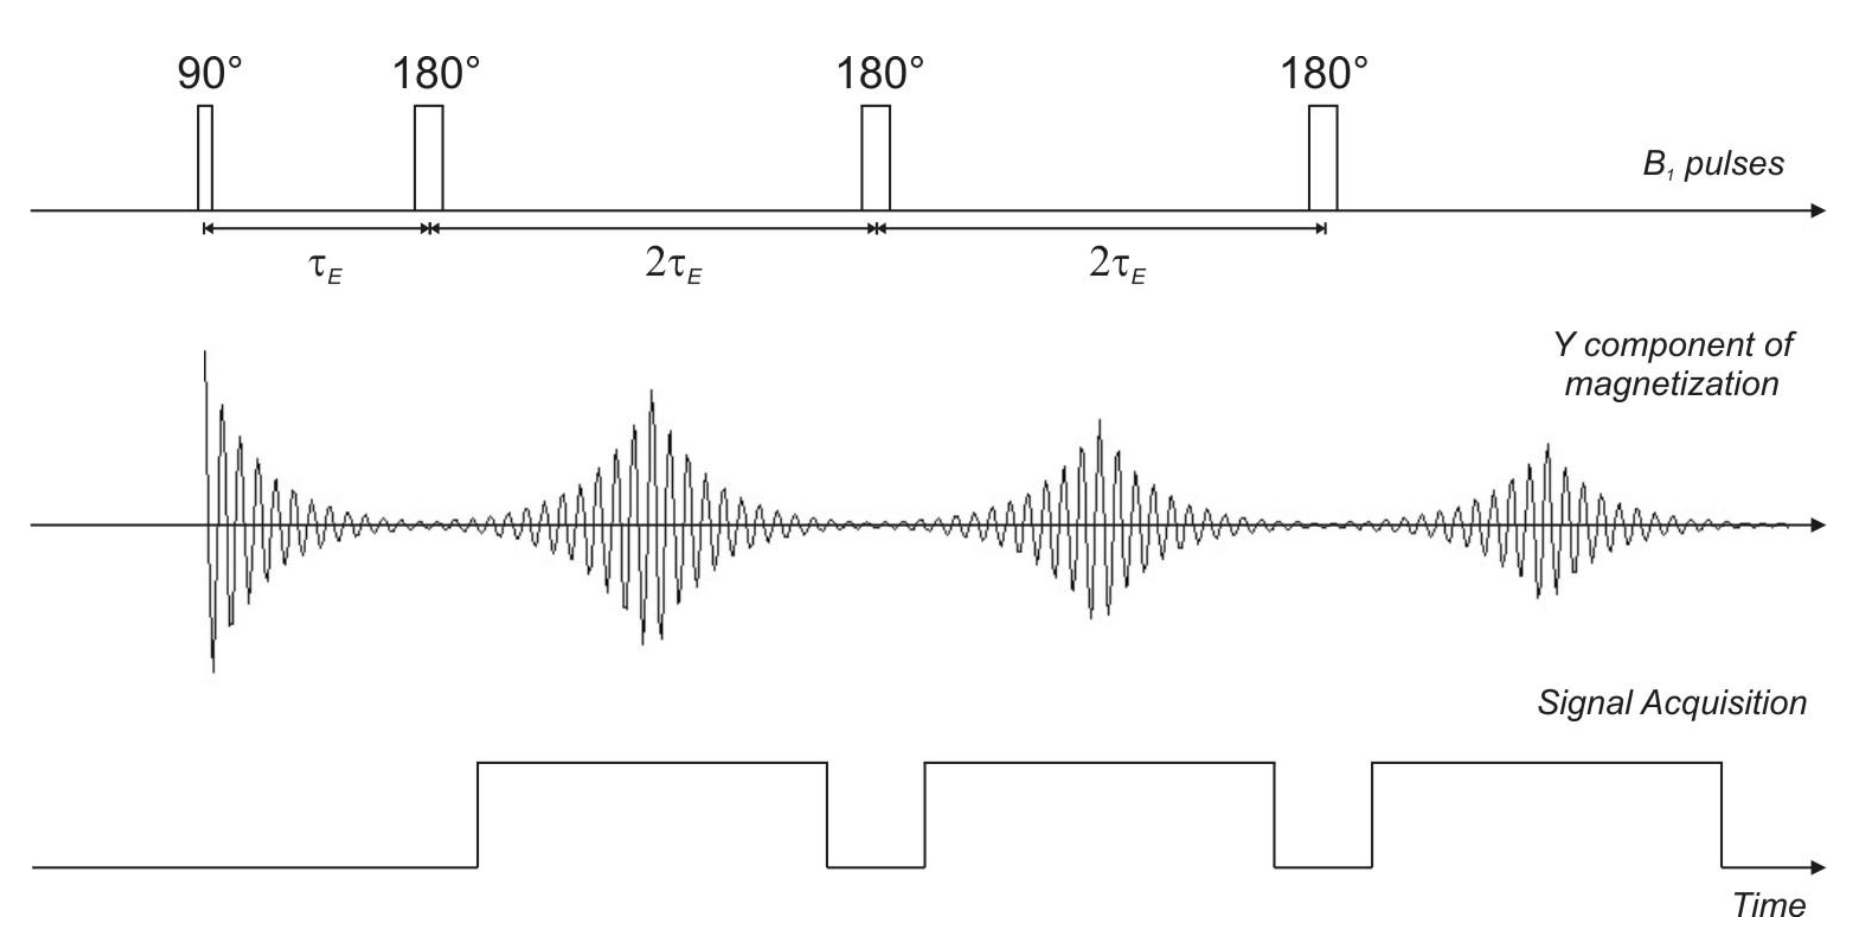
\includegraphics[width=11cm]{Bilddateien/10/CPMG_Prozess.png}
            \caption{Schaubildliche Darstellung des CPMG Prozesses. Die Zeit verläuft nach rechts, wohingegen die Systemantwort in Form des FIDs vertikal aufgetragen ist. Die blockweise Datensammlung ist Hardware- und softwareseitig festgelegt und zur $T_2$ Bestimmung verwendet. \cite[ch 5.3.1]{doc:EFNMRStudentManual}}
            \label{fig:CPMG-Prozess}
        \end{figure}

        Abhilfe schafft hier ein konstanter bzw. alternierender Phasenwinkel $\alpha$ zwischen dem initialen $\pi/2$ und den folgenen $\pi$ Pulsen (Car-Purcell-Meiboom-Gill Methode, CPMG). Dazu stellen wir in der Prospa Software die jeweiligen Phasenwinkel relativ zur Nullposition des einzelnen $\pi/2$ bzw. $\pi$ Pulses ein und berechnen die effektive Phasenverschiebung durch Subtraktion. Abbildung \ref{fig:CPMG_Parameter} zeigt dabei unsere verwendeten Parameter, die Phasenwinkel sind speziell unter \enquote{$90$ pulse phase (deg)} bzw. \enquote{$180$ pulse phase (deg)} zu finden \cite[ch 5.3]{doc:EFNMRStudentManual}.
        \begin{figure}[H]
            \centering
            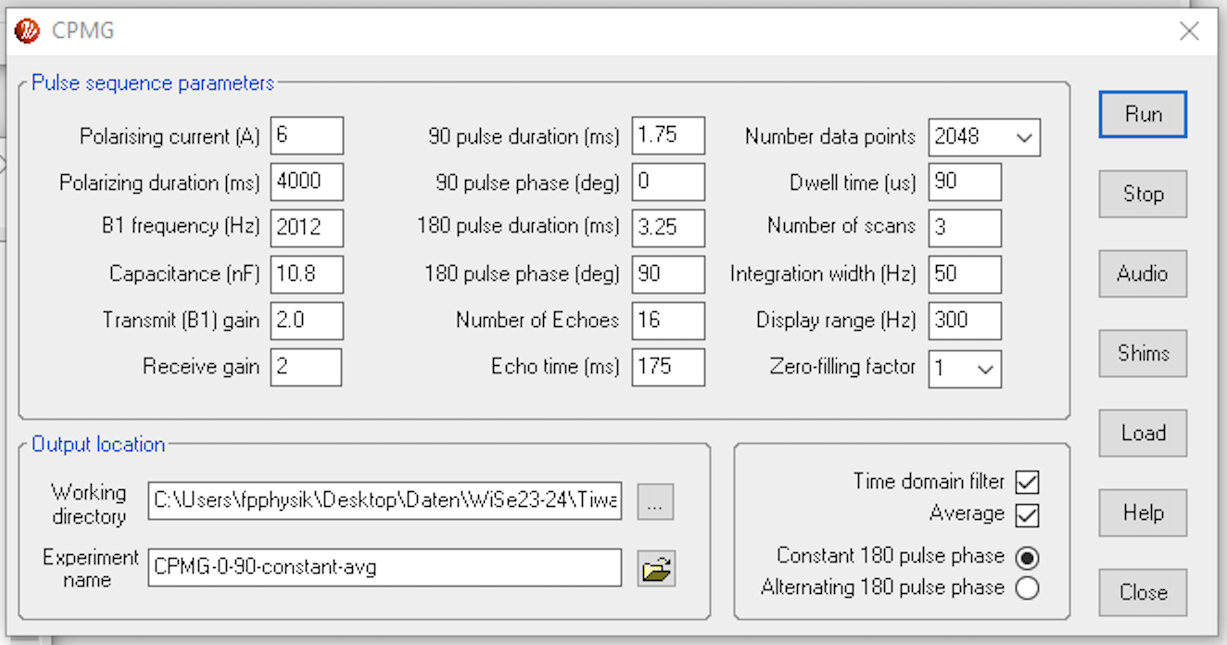
\includegraphics[width=11cm]{Bilddateien/10/CPMG_Parameter.png}
            \caption{Versuchsparameter zur Messung des CPMG Echos.}
            \label{fig:CPMG_Parameter}
        \end{figure}
        Nach konkreter Ausführung des Experimentes für einen Phasenwinkel $\alpha = 0$ erhält man bereits mit guten Parametern ein der Theorie entsprechendes Echobild, siehe Abbildung \ref{fig:sine-bell-func_example}. Da die effektive Phasenverschiebung lediglich in einer sinnvollen Menge $\{0,\pi/2,\pi,\pi/3\}$ durch Verschiebung um $\pi/2$ liegen sollte, können wir die Messergebnisse in kompakter Form in Tabelle \ref{tab:CPMG-avg} zusammenfassen. Bei der Messung haben wir dabei die Option der Mittelung im Kontrollfenster der Parameter (siehe Abb. \ref{fig:CPMG_Parameter}) aktiviert.
        \begin{figure}[H]
            \centering
            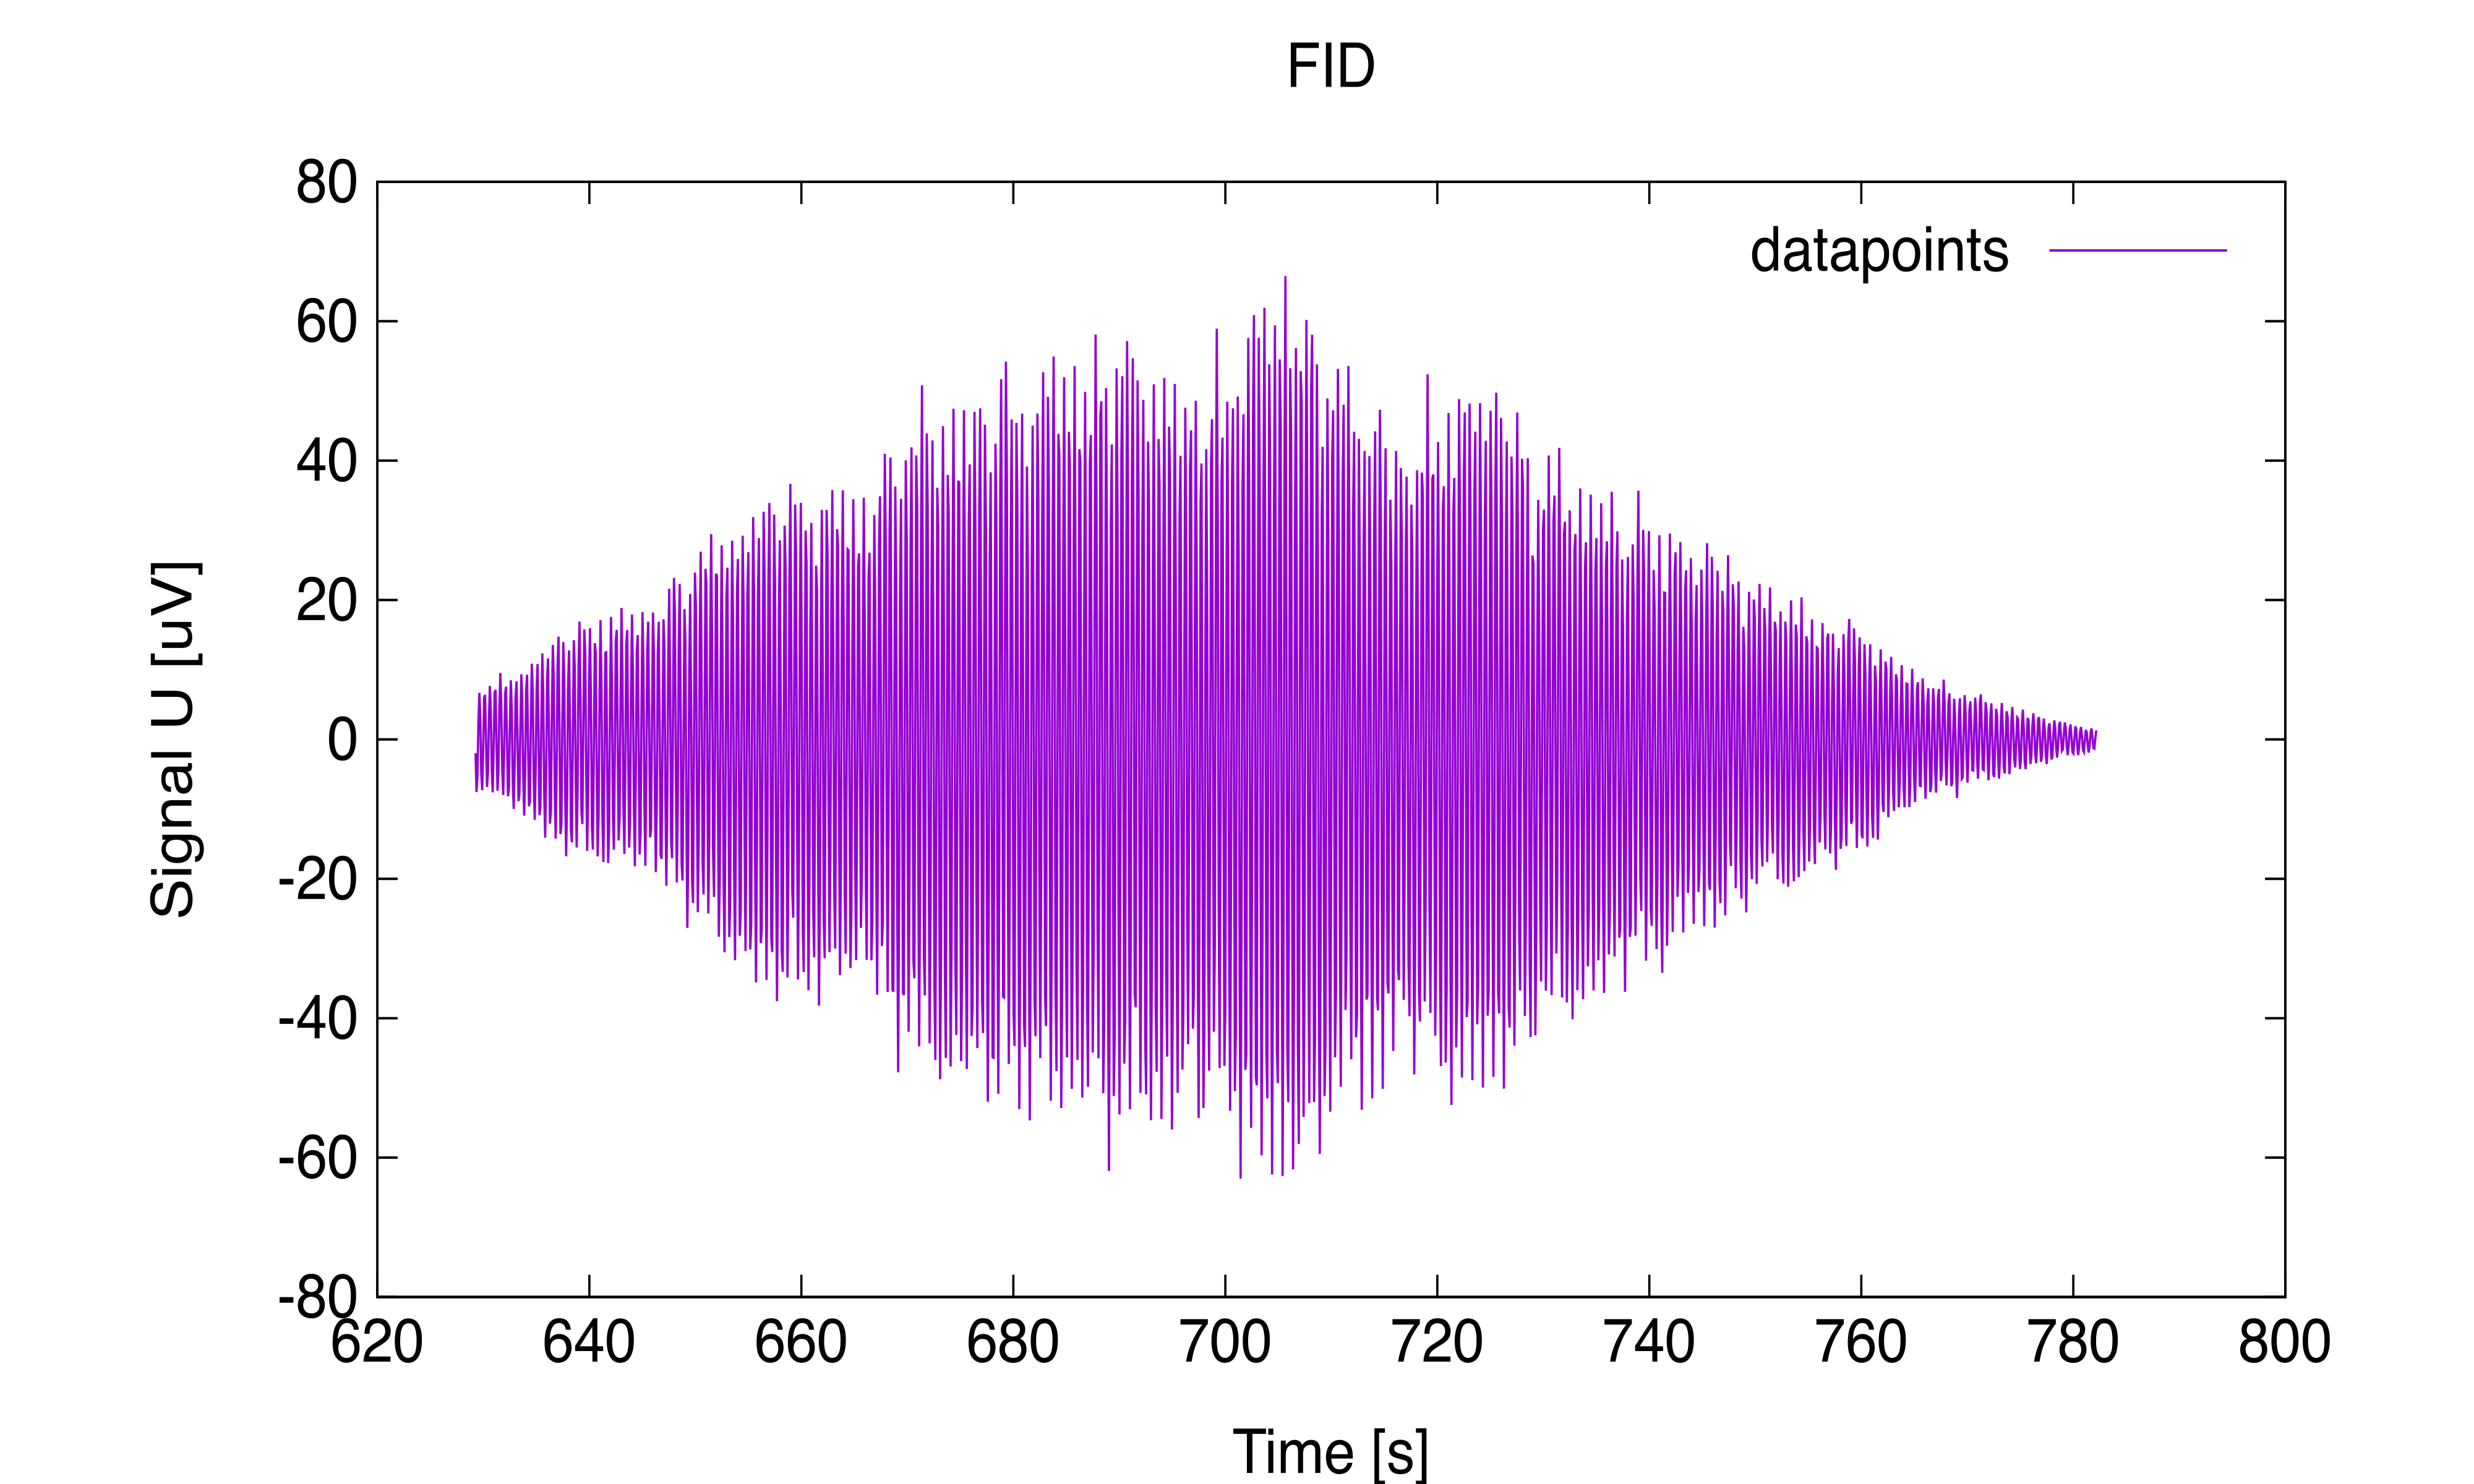
\includegraphics[width=11cm]{Bilddateien/10/sine-bell-func_example.png}
            \caption{Beispielverlauf des Echos, einer \emph{sine bell function} folgend. Die Phasenverschiebungen sind hier auf $0$ Grad gesetzt.}
            \label{fig:sine-bell-func_example} 
        \end{figure}

        \begin{table}[H]
            \centering
            \begin{tabular}{c|c|l|lll|l}
                $\varphi_1$ & $\varphi_2$ & mod. & $T_2$ in $\si{\ms}$ & $u(T_2)$ in $\si{\ms}$ & $T_2/u(T_2)$ in $\si{\percent}$ & ref. \\
                \hline\hline
                0 & 0 & const. & $1496.83$ & $220.1$ & $14.71$ & Abb. \ref{fig:CPMG-0-0-constant-avg} \\
                0 & 0 & alt. & $1850.27$ & $552.9$ & $29.88$ & Abb. \ref{fig:CPMG-0-0-alternating-avg} \\
                \hline
                0 & 90 & const. & $2317.43$ & $175.6$ & $7.58$ & Abb. \ref{fig:CPMG-0-90-constant-avg} \\
                0 & 90 & alt. & $590.08$ & $98.59$ & $16.71$ & Abb. \ref{fig:CPMG-0-90-alternating-avg} \\
                \hline
                0 & 180 & const. & $1439.91$ & $115.9$ & $8.05$ & Abb. \ref{fig:CPMG-0-180-constant-avg} \\
                0 & 180 & alt. & $1429.22$ & $185.3$ & $12.96$ & Abb. \ref{fig:CPMG-0-180-alternating-avg} \\
                \hline
                90 & 0 & const. & $1542.89$ & $110.7$ & $7.18$ & Abb. \ref{fig:CPMG-90-0-constant-avg} \\
                90 & 0 & alt. & $1072.73$ & $95.47$ & $8.89$ & Abb. \ref{fig:CPMG-90-0-alternating-avg} \\
                \hline
                180 & 0 & const. & $1070.47$ & $118.9$ & $11.11$ & Abb. \ref{fig:CPMG-180-0-constant-avg} \\
                180 & 0 & alt. & $1298.13$ & $212.6$ & $16.38$ & Abb. \ref{fig:CPMG-180-0-alternating-avg} \\
                \hline
                90 & 270 & const. & $533.729$ & $51.87$ & $9.72$ & Abb. \ref{fig:CPMG-90-270-constant-avg} \\
                90 & 270 & alt. & $1541.17$ & $245.1$ & $15.90$ & Abb. \ref{fig:CPMG-90-270-alternating-avg} \\
            \end{tabular}
            \caption{Gemittelte Auswirkungen der Pulsphasenwinkel auf die Relaxionszeit $T_2$ im Wasser.}
            \label{tab:CPMG-avg}
        \end{table}
        Die Berechnung der $T_2$ Zeiten erfolgt dabei softwareseitig durch implementierte Fouriertransformation des einzelnen Echopeaks (siehe Abb. \ref{fig:sine-bell-func_example}) unter Verwendung des ebenfalls softwareseitig festgelegten Datenerfassungszeitfenster, in Abbildung \ref{fig:CPMG-Prozess} unter \enquote{acquisition time} der \enquote{Signal acquisition} Blöcke identifizierbar. Als alternativer Weg wird die Bestimmung der Intensität des Peakmaximums jedes Echos angegeben, jedoch weist die Integrationsmethode rauschunterdrückende Eigenschaften auf, sodaß wir die softwareseitige Implementierung verwenden \cite[ch 5.3.1]{doc:EFNMRStudentManual}. 
        \subsubsection*{Dateninterpretation}
            Die erste Annahme, welche durch unsere Messungen widerlegt wird, ist die Symmetrie der effektiven Phasenverschiebung $\alpha$ für beliebige Winkelpaare $(\varphi_1,\varphi_2)$ mit $\abs{\varphi_1 - \varphi_2} = \pi/2$, bzw. $\abs{\varphi_1 - \varphi_2} = \pi$ oder $\abs{\varphi_1 - \varphi_2} = 3\pi/2$. Es zeigt sich hier beispielsweise bei $(\pi/2,0)$ bzw. $(0,\pi/2)$ bei konstanter Phasenverschiebung für die $T_1$ Zeit das Ergebnis
            \[
                T_1^{\textit{const}}(\pi/2,0) = 1542.89(11070)\si{\ms},\qquad T_1^{\textit{const}}(0,\pi/2) = 2317.43(17560)\si{\ms}.
            \]
            Dabei liegt selbst im angegebenen Unsicherheitsbereich keine Überschneidung vor. 

            Weiter fällt deutlich auf, dass bei einer Nullverschiebung $\alpha = 0$ bei konstanter bzw. alternierender Variierung ungleiche Ergebnisse gemessen werden. Dies ist physikalisch nicht plausibel, lässt sich jedoch mit überlappenden Unsicherheitsbereichen korrigieren:
            \[
                T_2^{\textit{const}}(0,0) = 1496.83(22010)\si{\ms},\qquad T_2^{\textit{alt}}(0,0) = 1850.27(55290)\si{\ms}.
            \]
            Generell liegen bei alternierenden Messreihen höhere Unsicherheiten vor, wie durch die prozentuale Darstellung in Tabelle \ref{tab:CPMG-avg} deutlich wird. 

            Bei einer Phasenverschiebung von $\pi$ ähneln sich die Werte $T_2^{\textit{const}}(0,0)$ und $T_2^{\textit{const}}(0,180)$ stark, jedoch nicht $T_2^{\textit{const}}(180,0)$ wegen ausbleibender diskutierter Symmetrie. Auch $T_2^{\textit{const}}(90,270)$ ist in keinster Weise vereinbar mit den zu $\alpha = \pi$ gehörigen Werten. Im Bereich der alternierenden Messergebnisse überlappen sich die Unsicherheitsintervalle von $T_2^{\textit{alt}}(0,0)$ und $T_2^{\textit{alt}}(0,180)$ aufgrund des großen Unsicherheitsradius $u(T_2^{\textit{alt}}(0,0))$. Optisch kann man diesen bereits aus der zugehörigen Abbildung \ref{fig:CPMG-0-0-alternating-avg} durch die hohe Variation der Messpunkte um die exponentielle Kurvenanpassung entnehmen.
            %Dies ist physikalisch plausibel, da 
            
            Vergleicht man pro Tupelwahl $(\varphi_1,\varphi_2)$ die jeweiligen $T_1^{\textit{const}}$ und $T_1^{\textit{alt}}$ Werte, so fällt leider ebenfalls kein deutliches Muster auf. 

            Unseren maximal gemessenen Wert $T_2$ finden wir in der konstanten $\alpha = \pi$ Phasenverschiebung vor, wie auch unser zweites Minimum.

            In den folgenden Grafiken \ref{fig:CPMG-0-0-alternating-avg} bis \ref{fig:CPMG-90-270-alternating-avg} sind die gemittelten FIDs und Amplitudensignale für die jeweiligen Phasenwinkel $\varphi_1$ und $\varphi_2$ nichtnormiert aufgetragen. Dabei wurden die Amplituden mit der $T_2$ decay time gewichtet durch die Software berechnet \cite[ch 5.3.1]{doc:EFNMRStudentManual}. Die Messwerte wurden dabei mit der Kurvenfunktion 
            \[
                f(x,a,b,c) = a\cdot \exp(-\frac{x}{b}) + c
            \]
            angenähert, sodass man durch $b$ bereits direkt die Relaxionszeit $T_2$ ablesen kann. 
        \begin{figure}[H]
            \centering
            \begin{subfigure}[b]{0.4\textwidth}
                \centering
                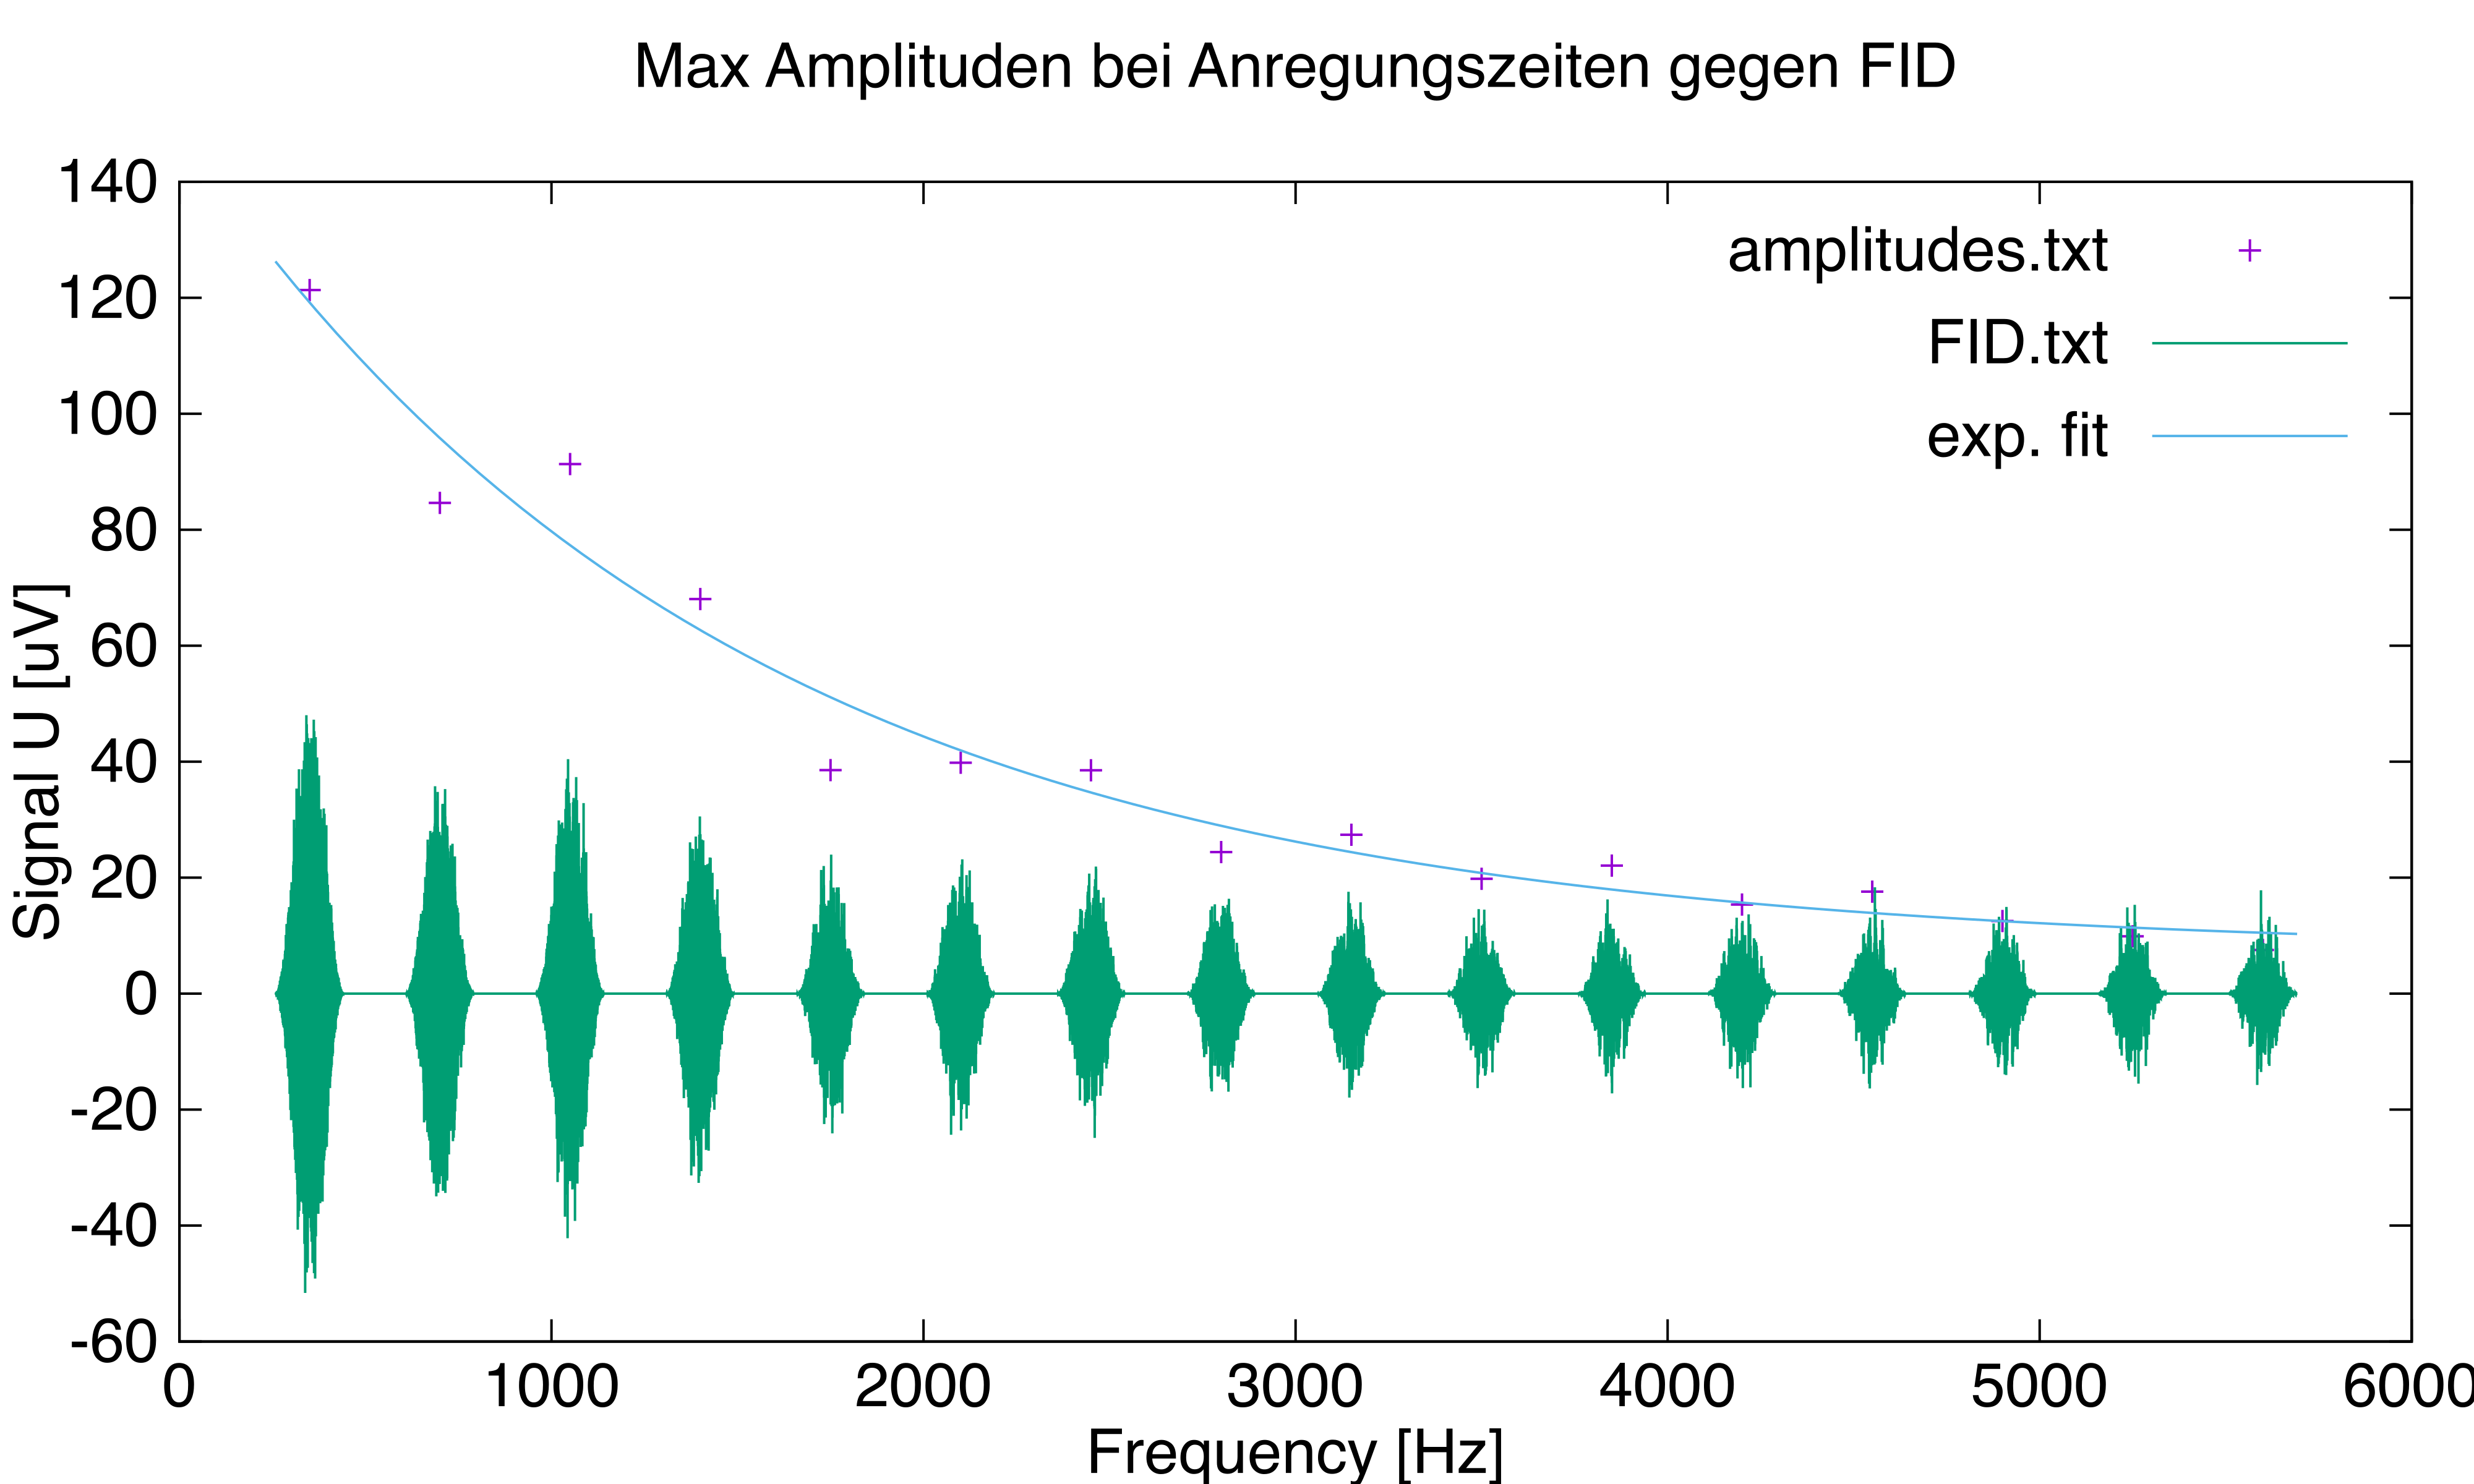
\includegraphics[width=6cm]{Bilddateien/10/CPMG-0-0-constant-avg.png}
                \caption{mod. const.}
                \label{fig:CPMG-0-0-constant-avg}
            \end{subfigure}
            \
            \begin{subfigure}[b]{0.4\textwidth}
                \centering
                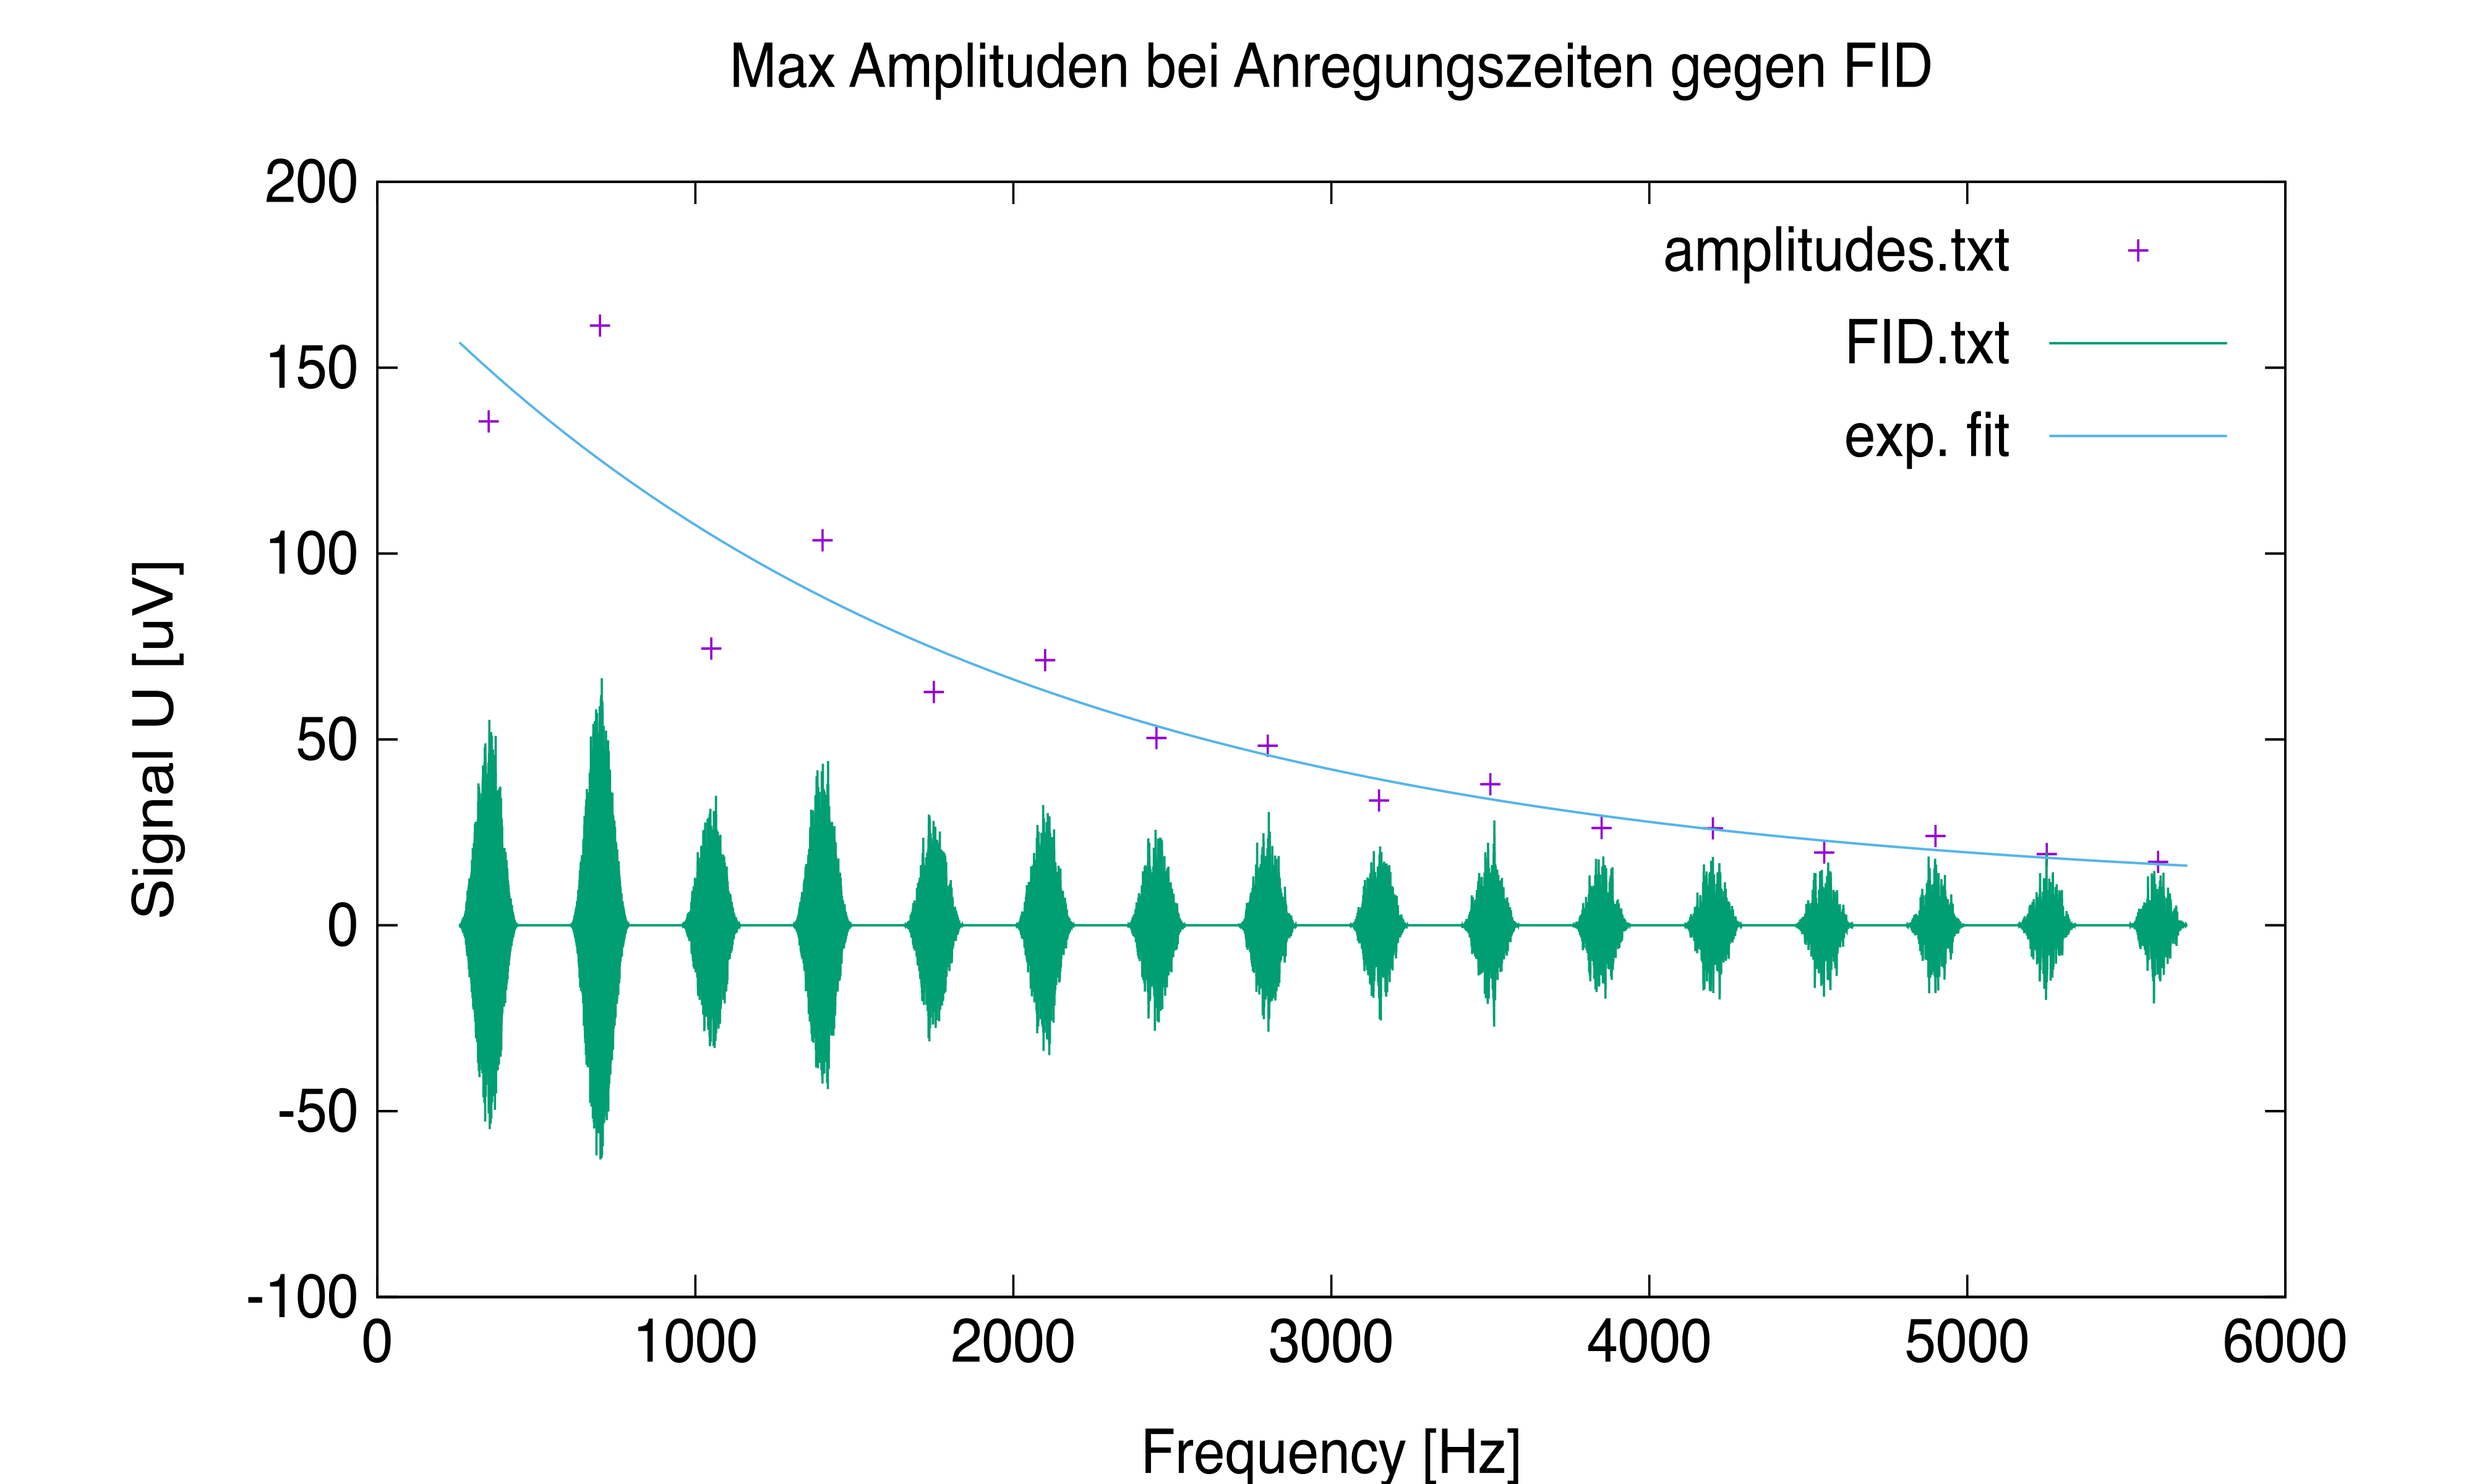
\includegraphics[width=6cm]{Bilddateien/10/CPMG-0-0-alternating-avg.png}
                \caption{mod. alt.}
                \label{fig:CPMG-0-0-alternating-avg}
            \end{subfigure}
            \caption{FID und Amplitudensignale nichtnormiert und gemittelt für $\varphi_1 = 0$, $\varphi_2 = 0$.}
            \label{fig:CPMG-0-0-avg}
        \end{figure}

        \begin{figure}[H]
            \centering
            \begin{subfigure}[b]{0.4\textwidth}
                \centering
                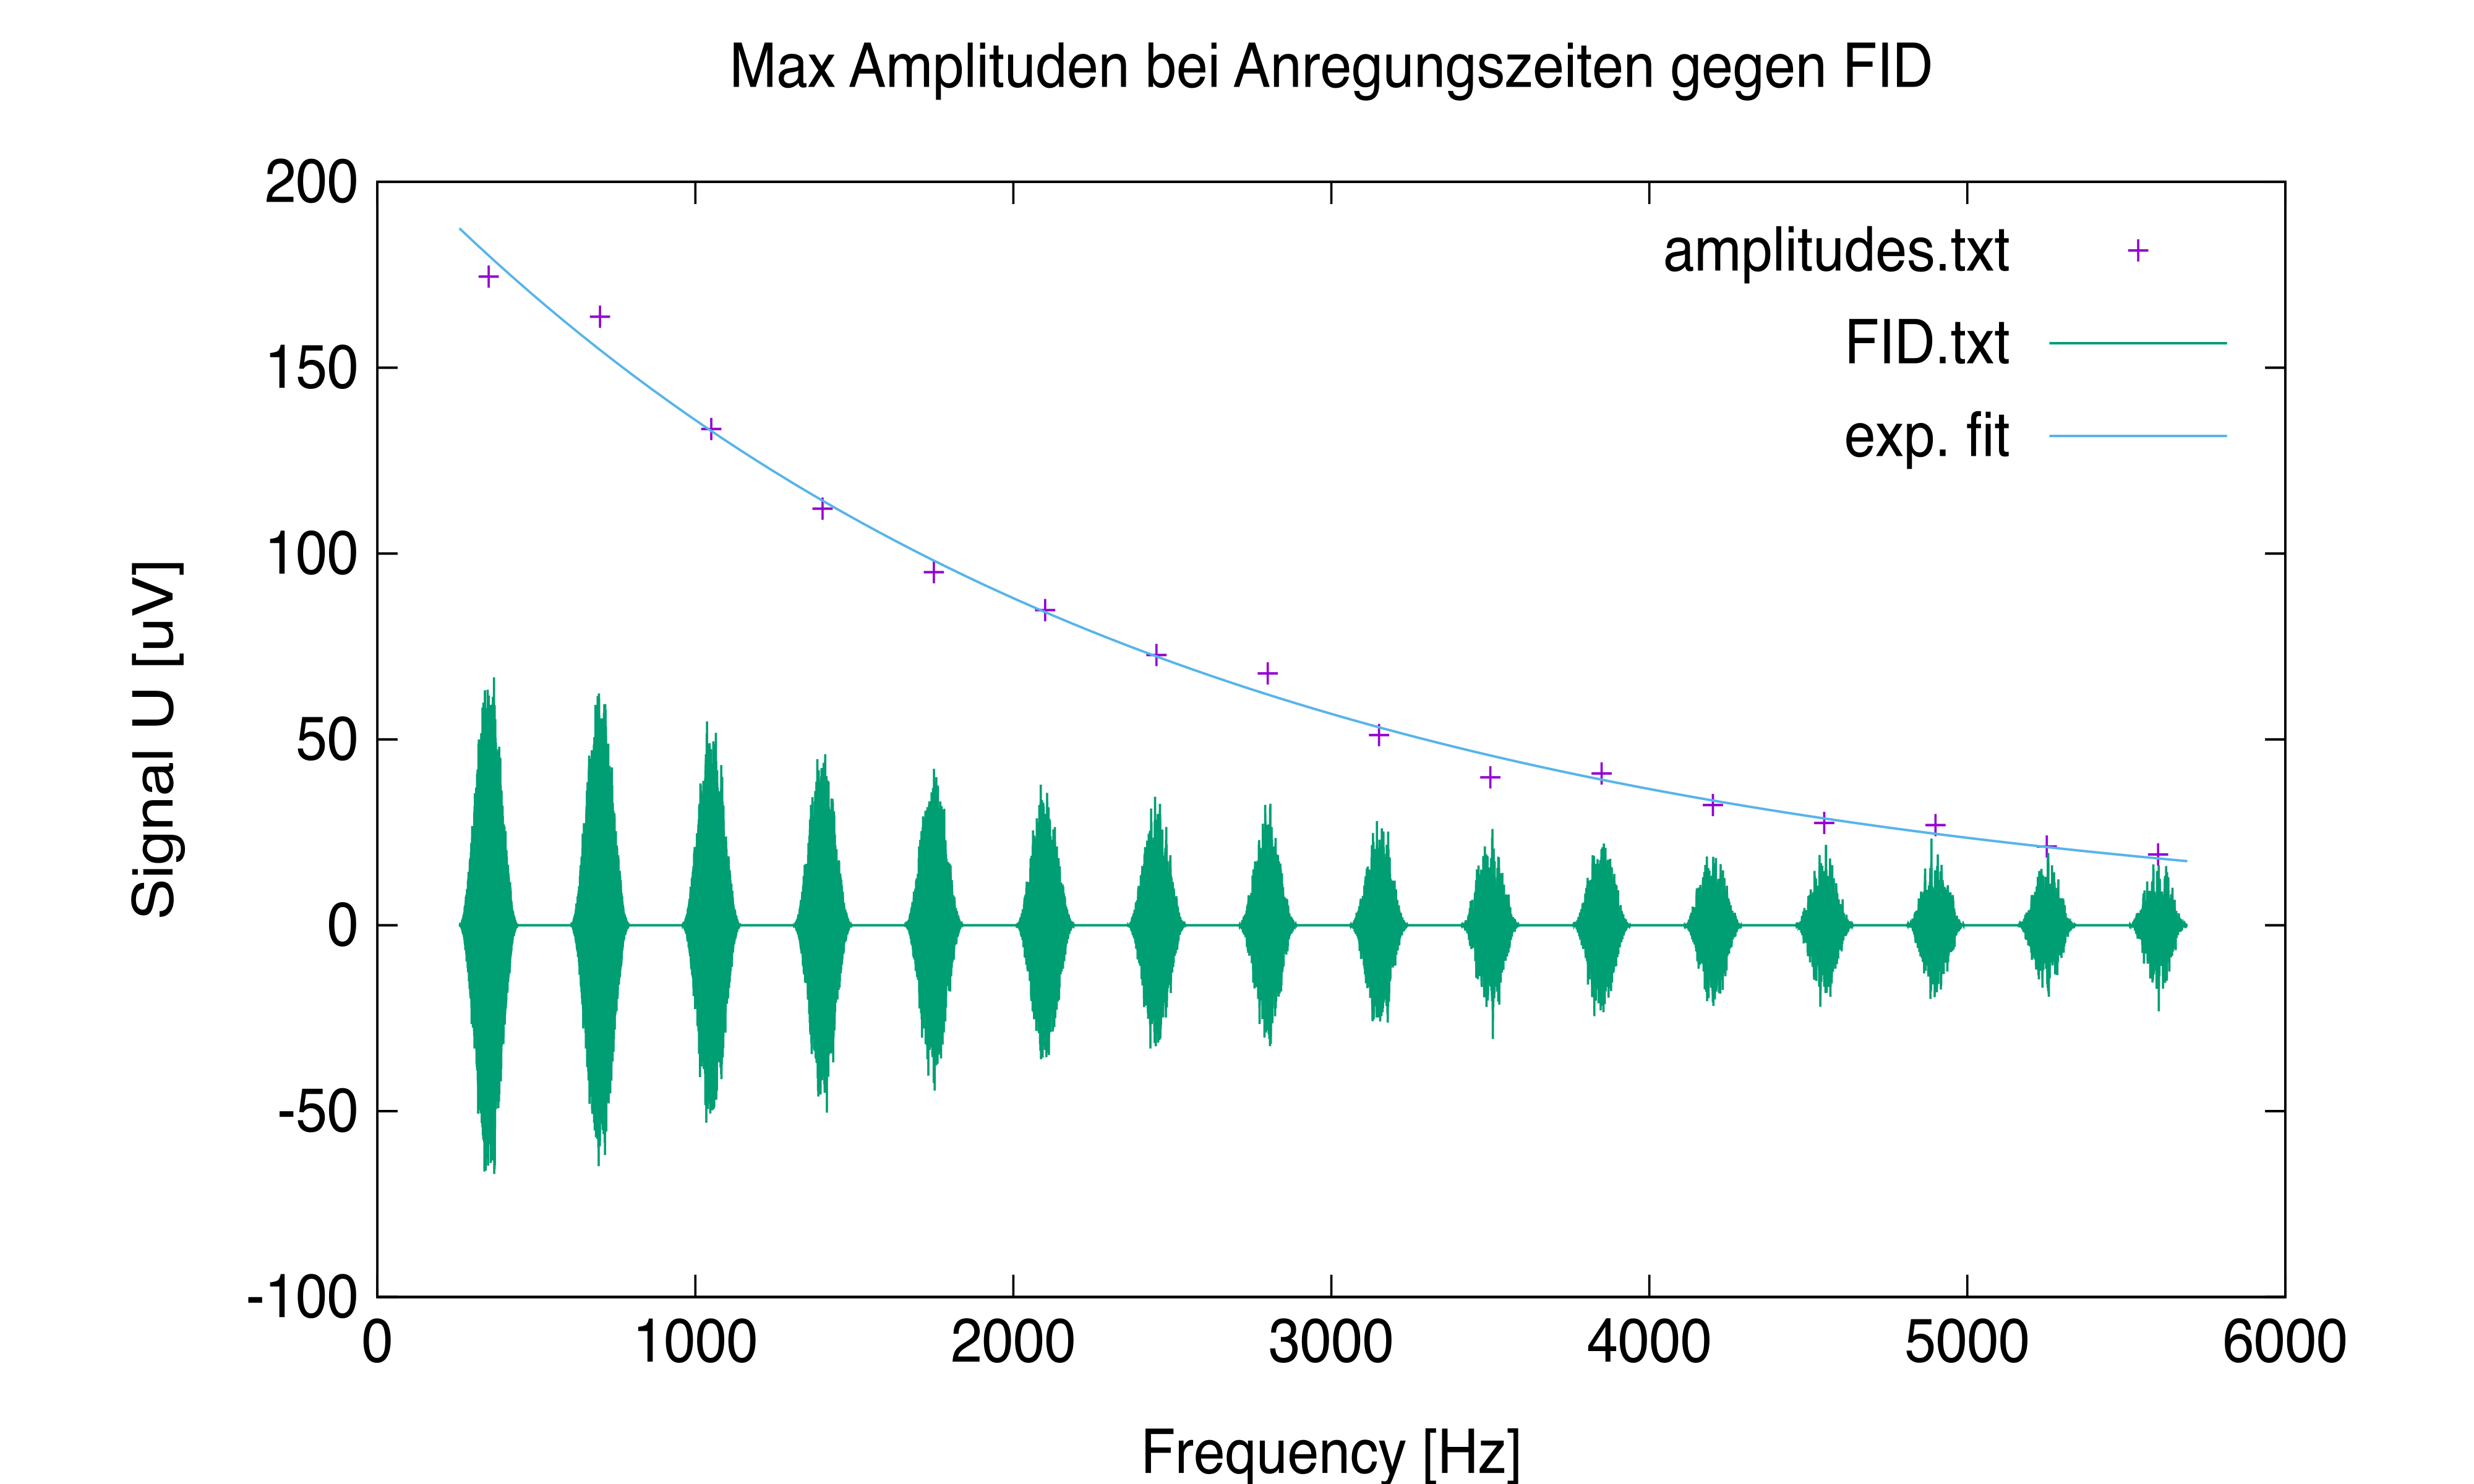
\includegraphics[width=6cm]{Bilddateien/10/CPMG-0-90-constant-avg.png}
                \caption{mod. const.}
                \label{fig:CPMG-0-90-constant-avg}
            \end{subfigure}
            \
            \begin{subfigure}[b]{0.4\textwidth}
                \centering
                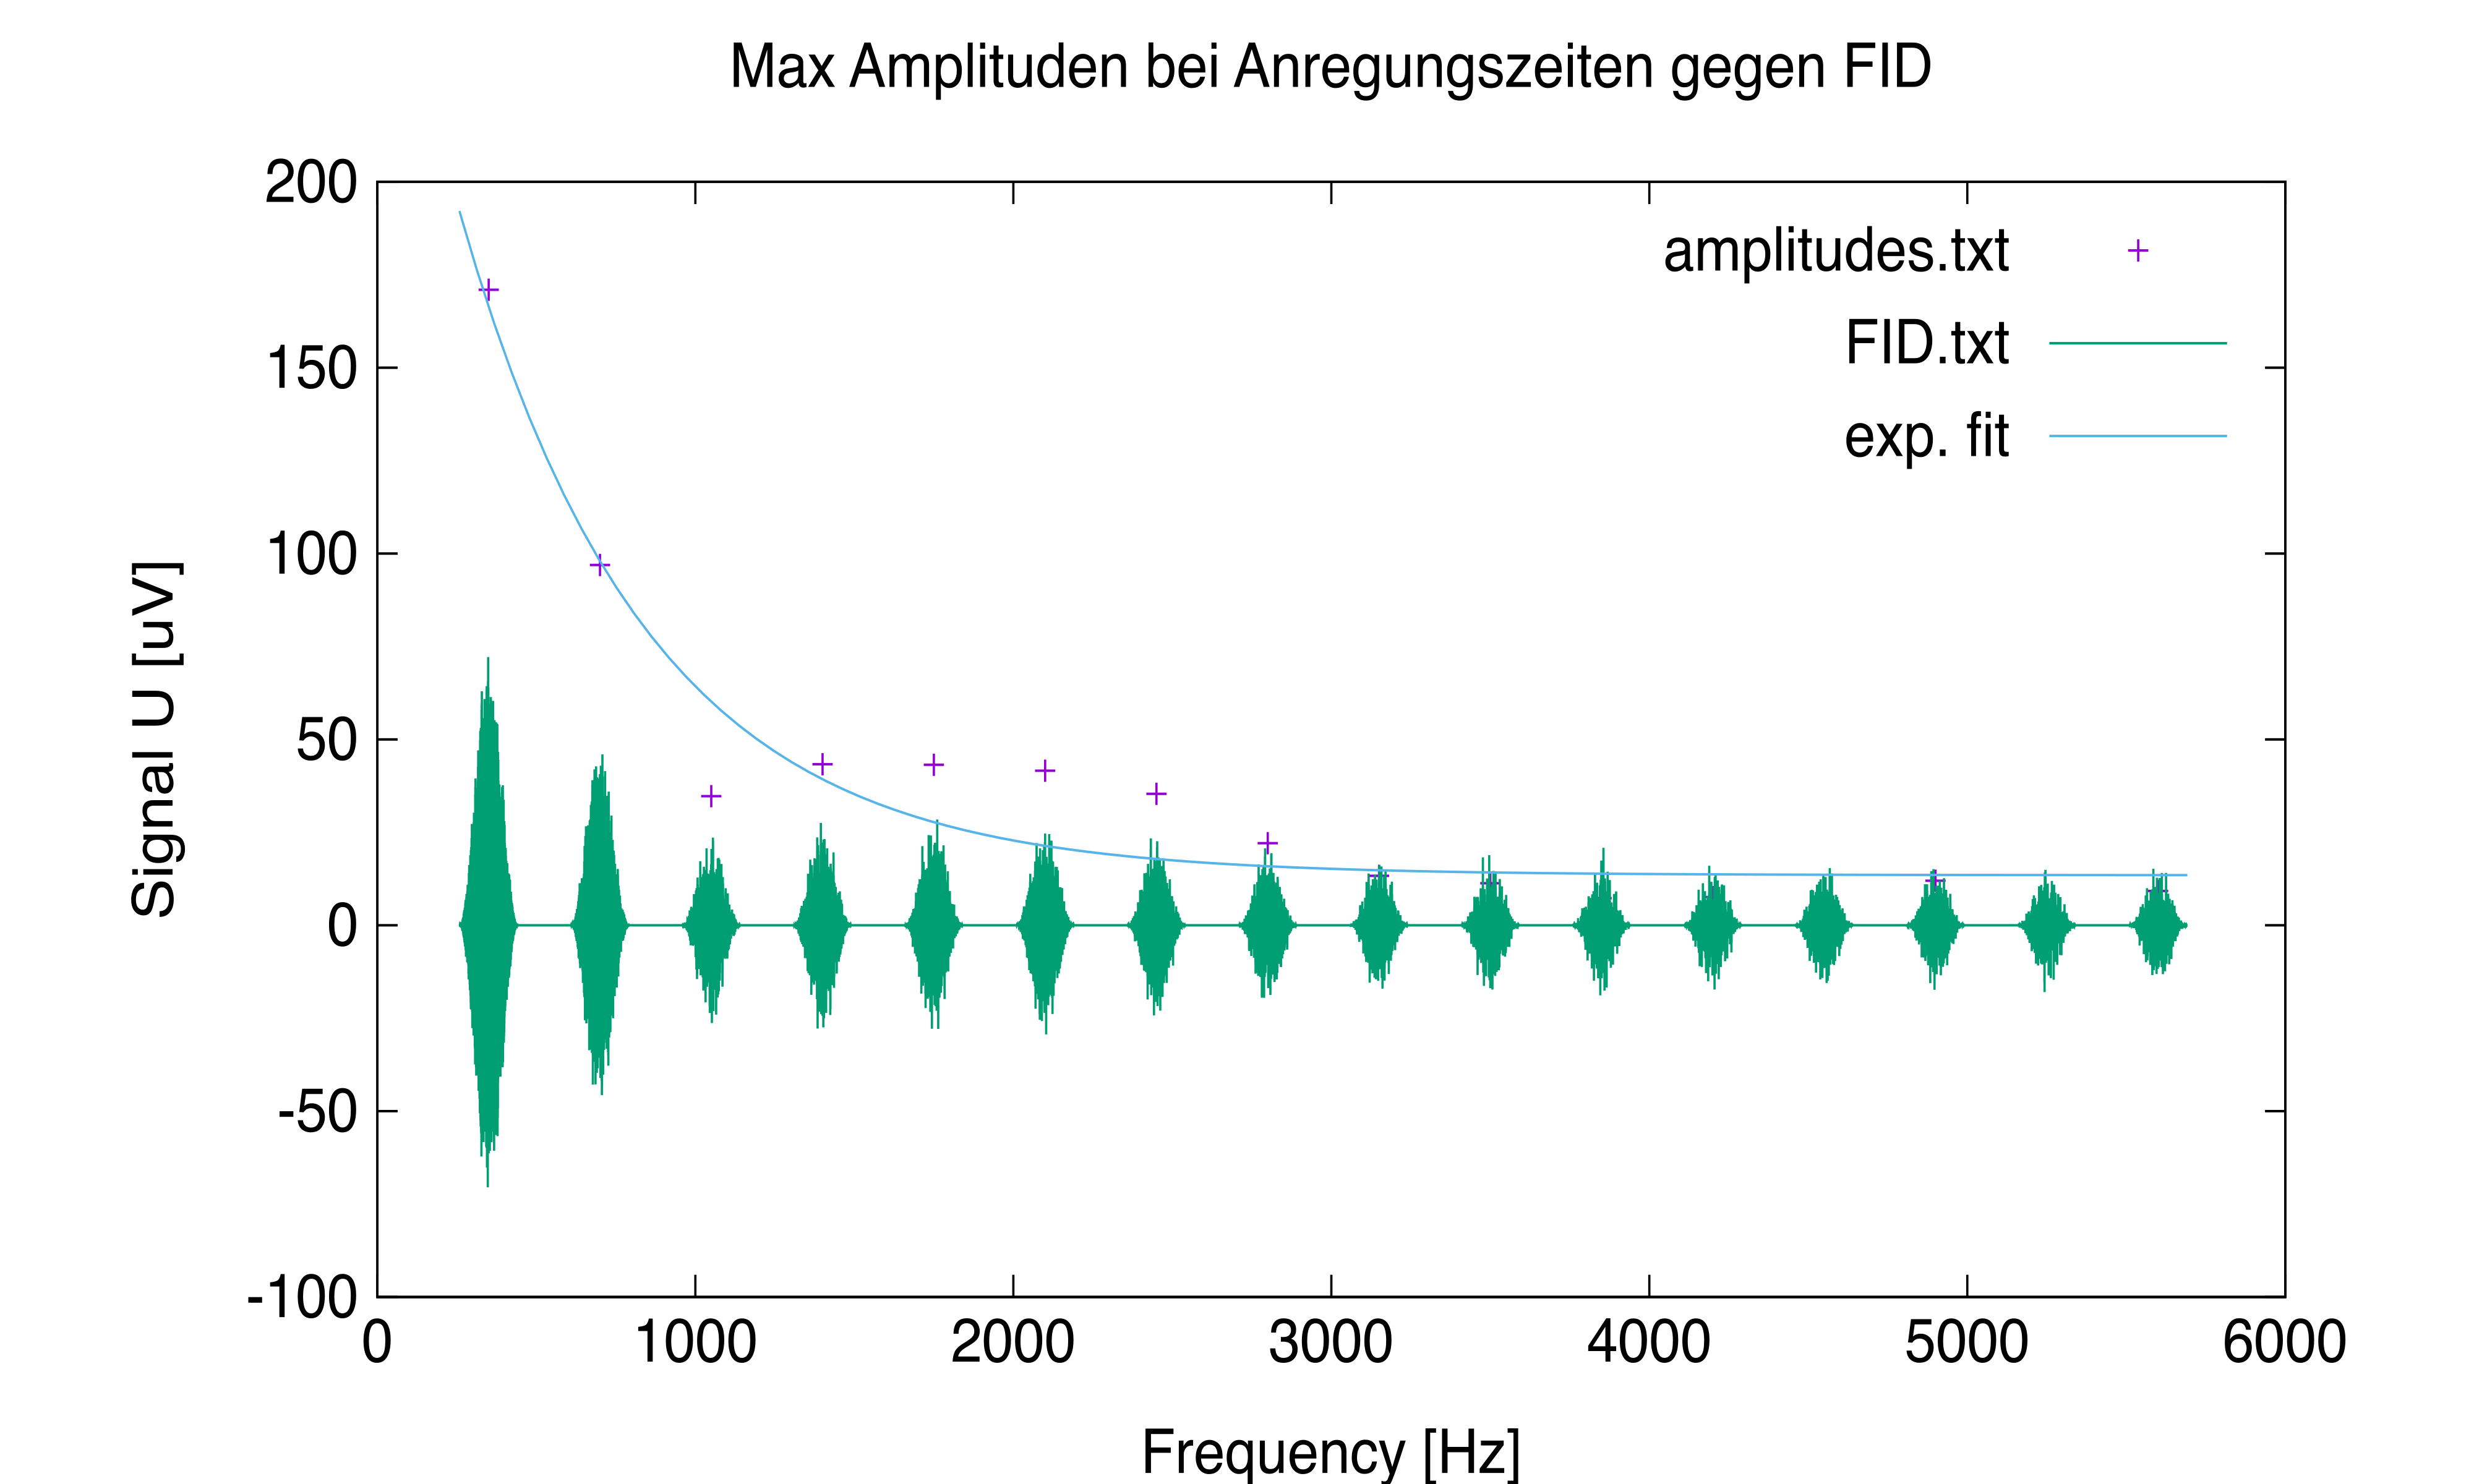
\includegraphics[width=6cm]{Bilddateien/10/CPMG-0-90-alternating-avg.png}
                \caption{mod. alt.}
                \label{fig:CPMG-0-90-alternating-avg}
            \end{subfigure}
            \caption{FID und Amplitudensignale nichtnormiert und gemittelt für $\varphi_1 = 0$, $\varphi_2 = 90$.}
            \label{fig:CPMG-0-90-avg}
        \end{figure}
        
        \begin{figure}[H]
            \centering
            \begin{subfigure}[b]{0.4\textwidth}
                \centering
                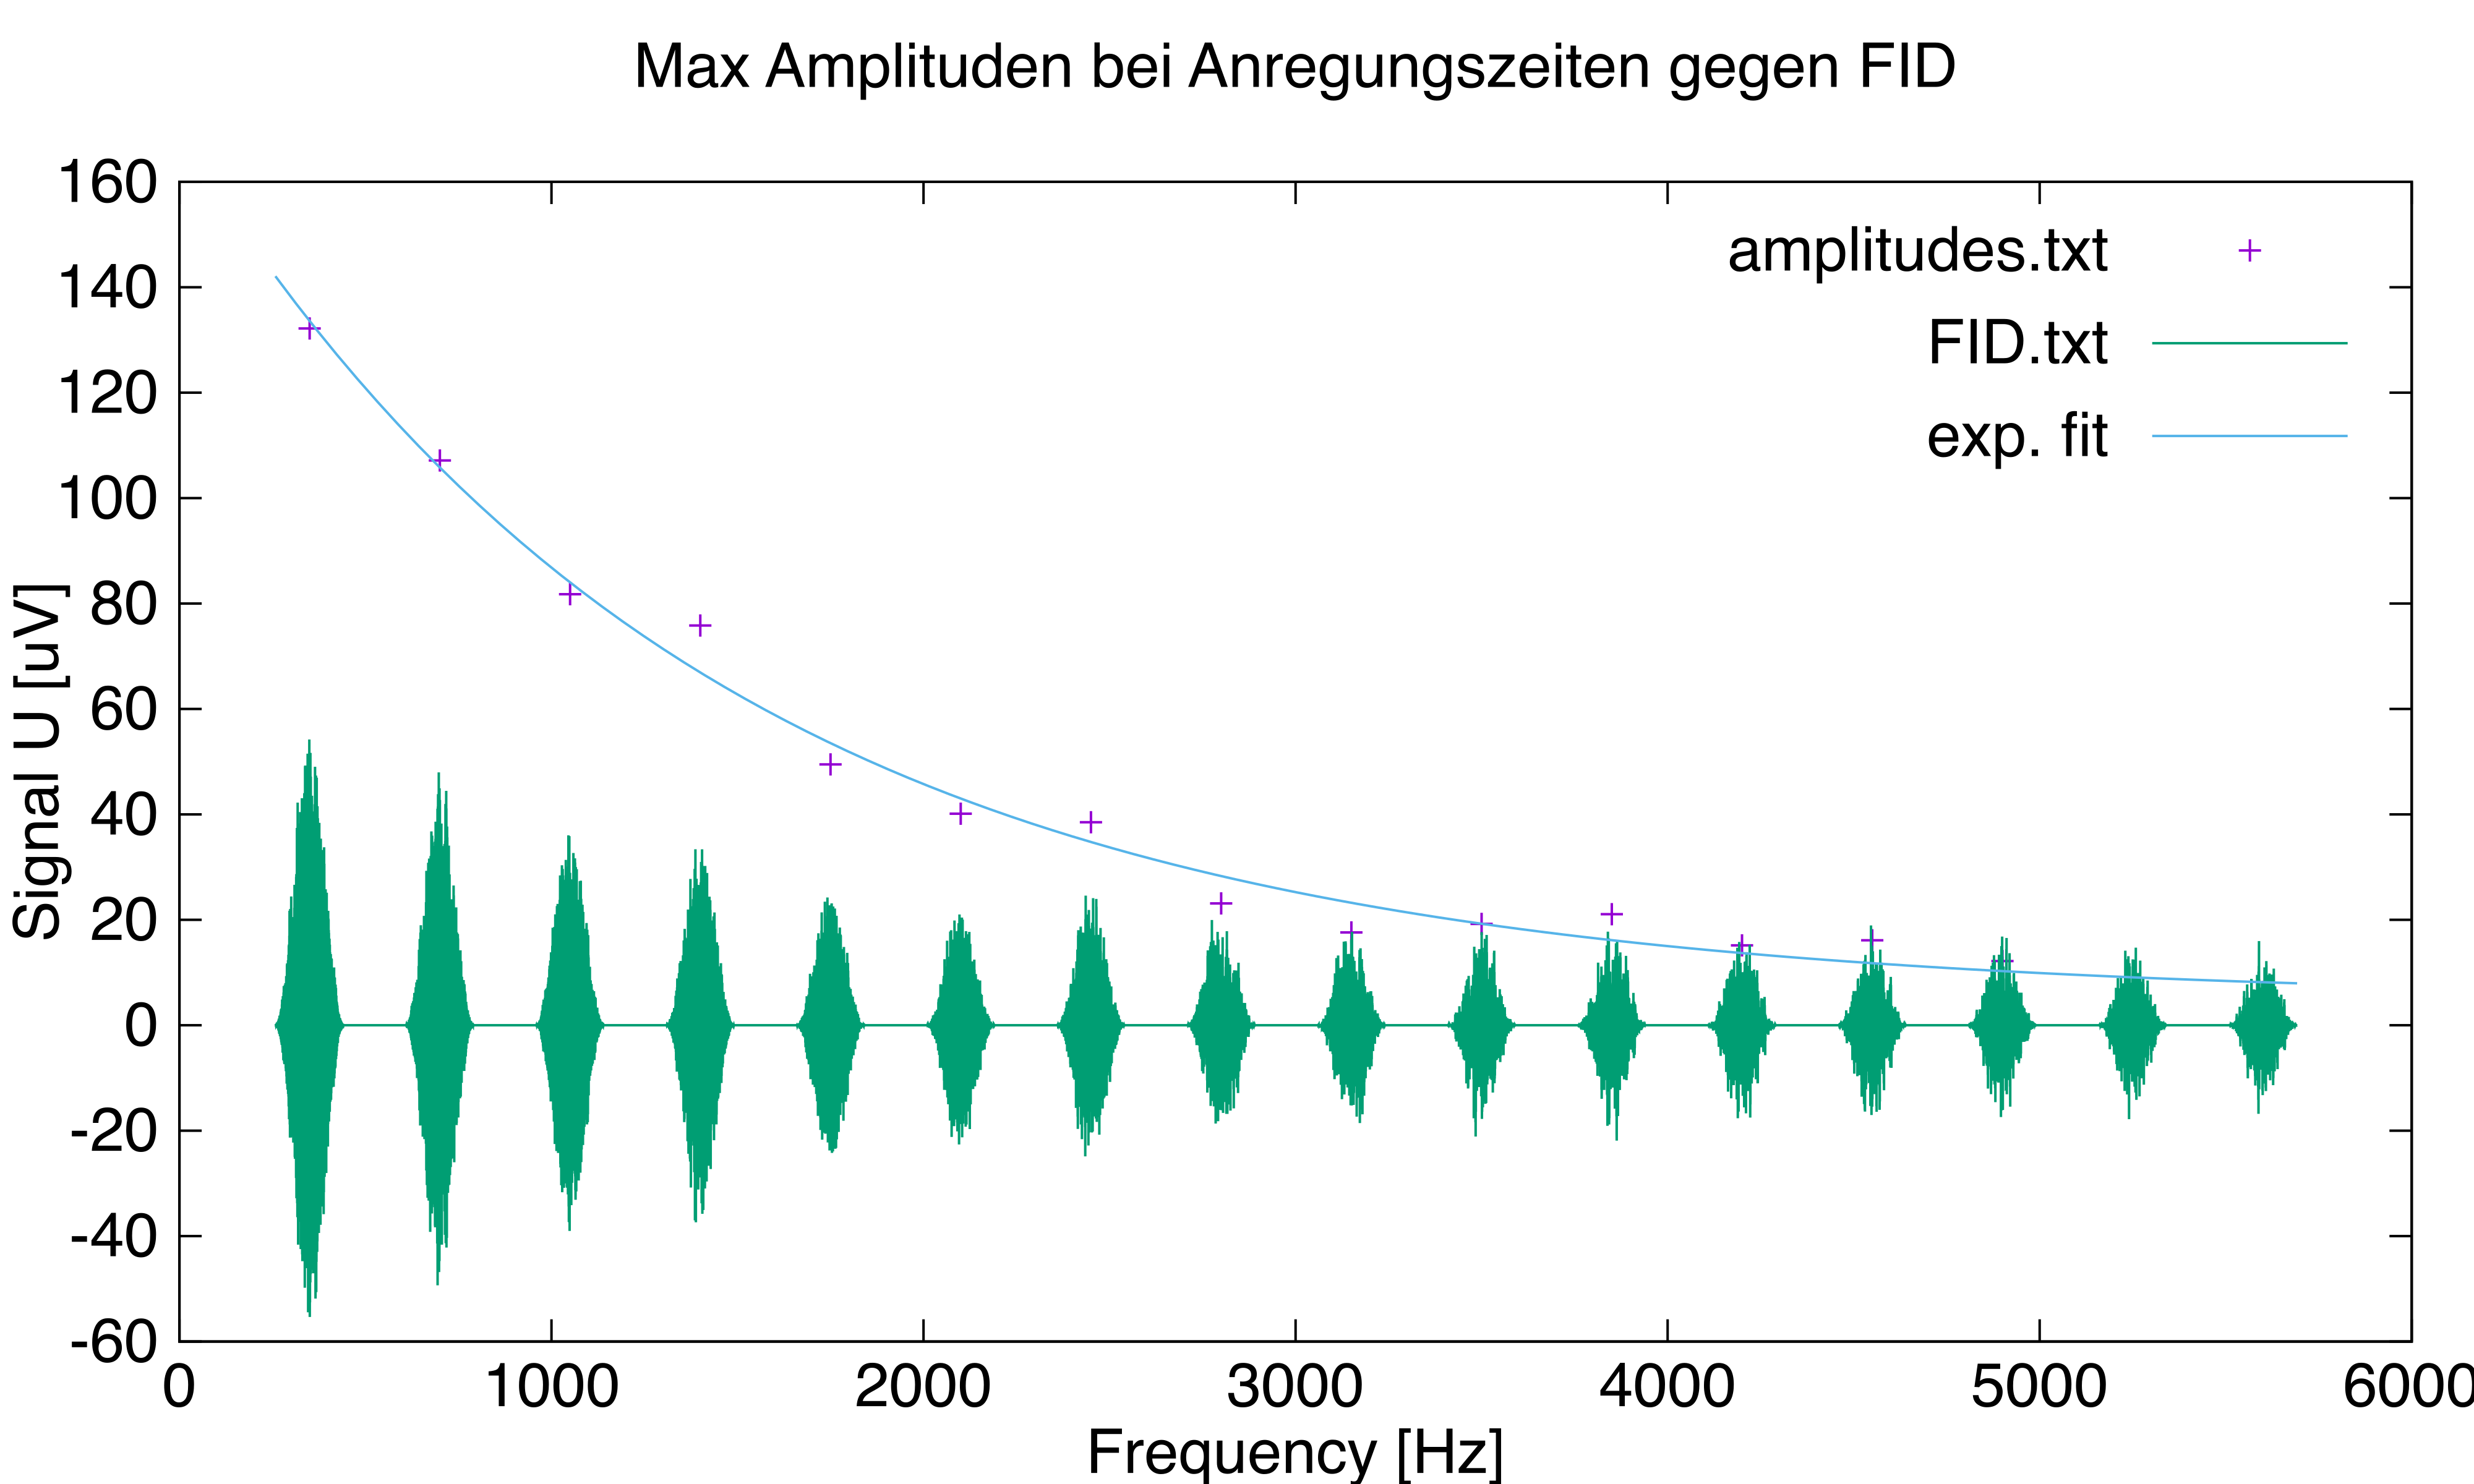
\includegraphics[width=6cm]{Bilddateien/10/CPMG-0-180-constant-avg.png}
                \caption{mod. const.}
                \label{fig:CPMG-0-180-constant-avg}
            \end{subfigure}
            \
            \begin{subfigure}[b]{0.4\textwidth}
                \centering
                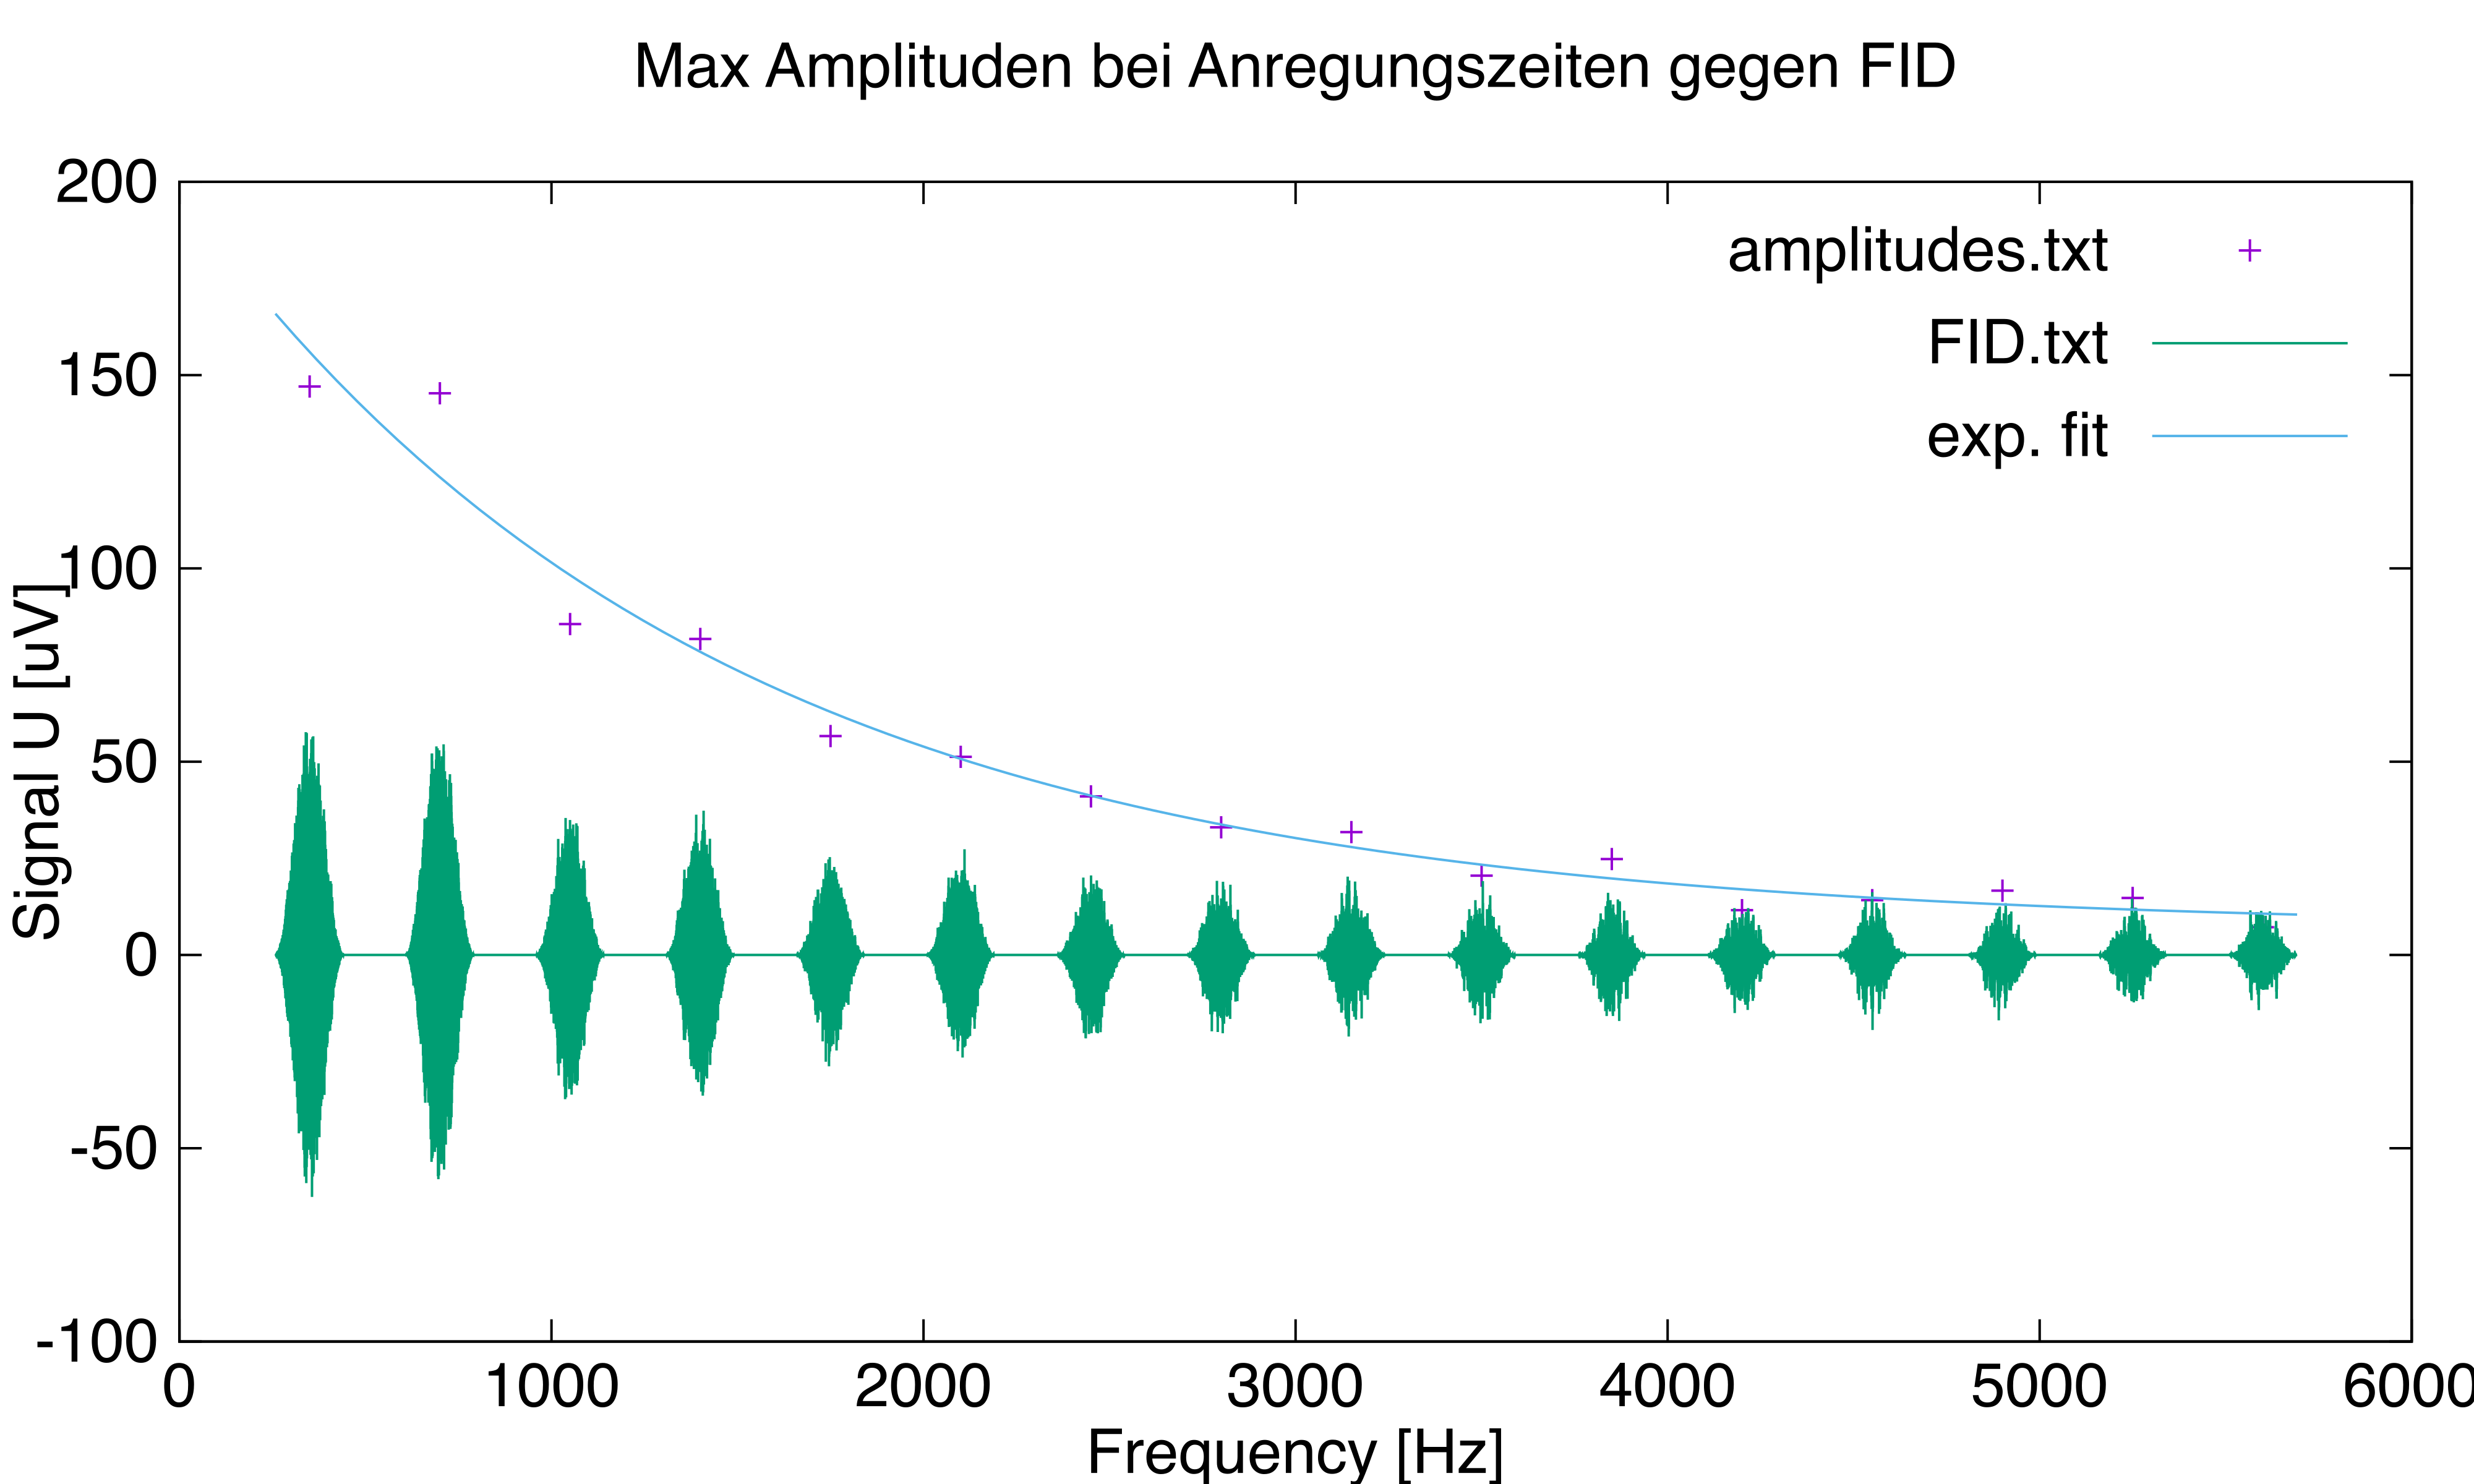
\includegraphics[width=6cm]{Bilddateien/10/CPMG-0-180-alternating-avg.png}
                \caption{mod. alt.}
                \label{fig:CPMG-0-180-alternating-avg}
            \end{subfigure}
            \caption{FID und Amplitudensignale nichtnormiert und gemittelt für $\varphi_1 = 0$, $\varphi_2 = 180$.}
            \label{fig:CPMG-0-180-avg}
        \end{figure}

        \begin{figure}[H]
            \centering
            \begin{subfigure}[b]{0.4\textwidth}
                \centering
                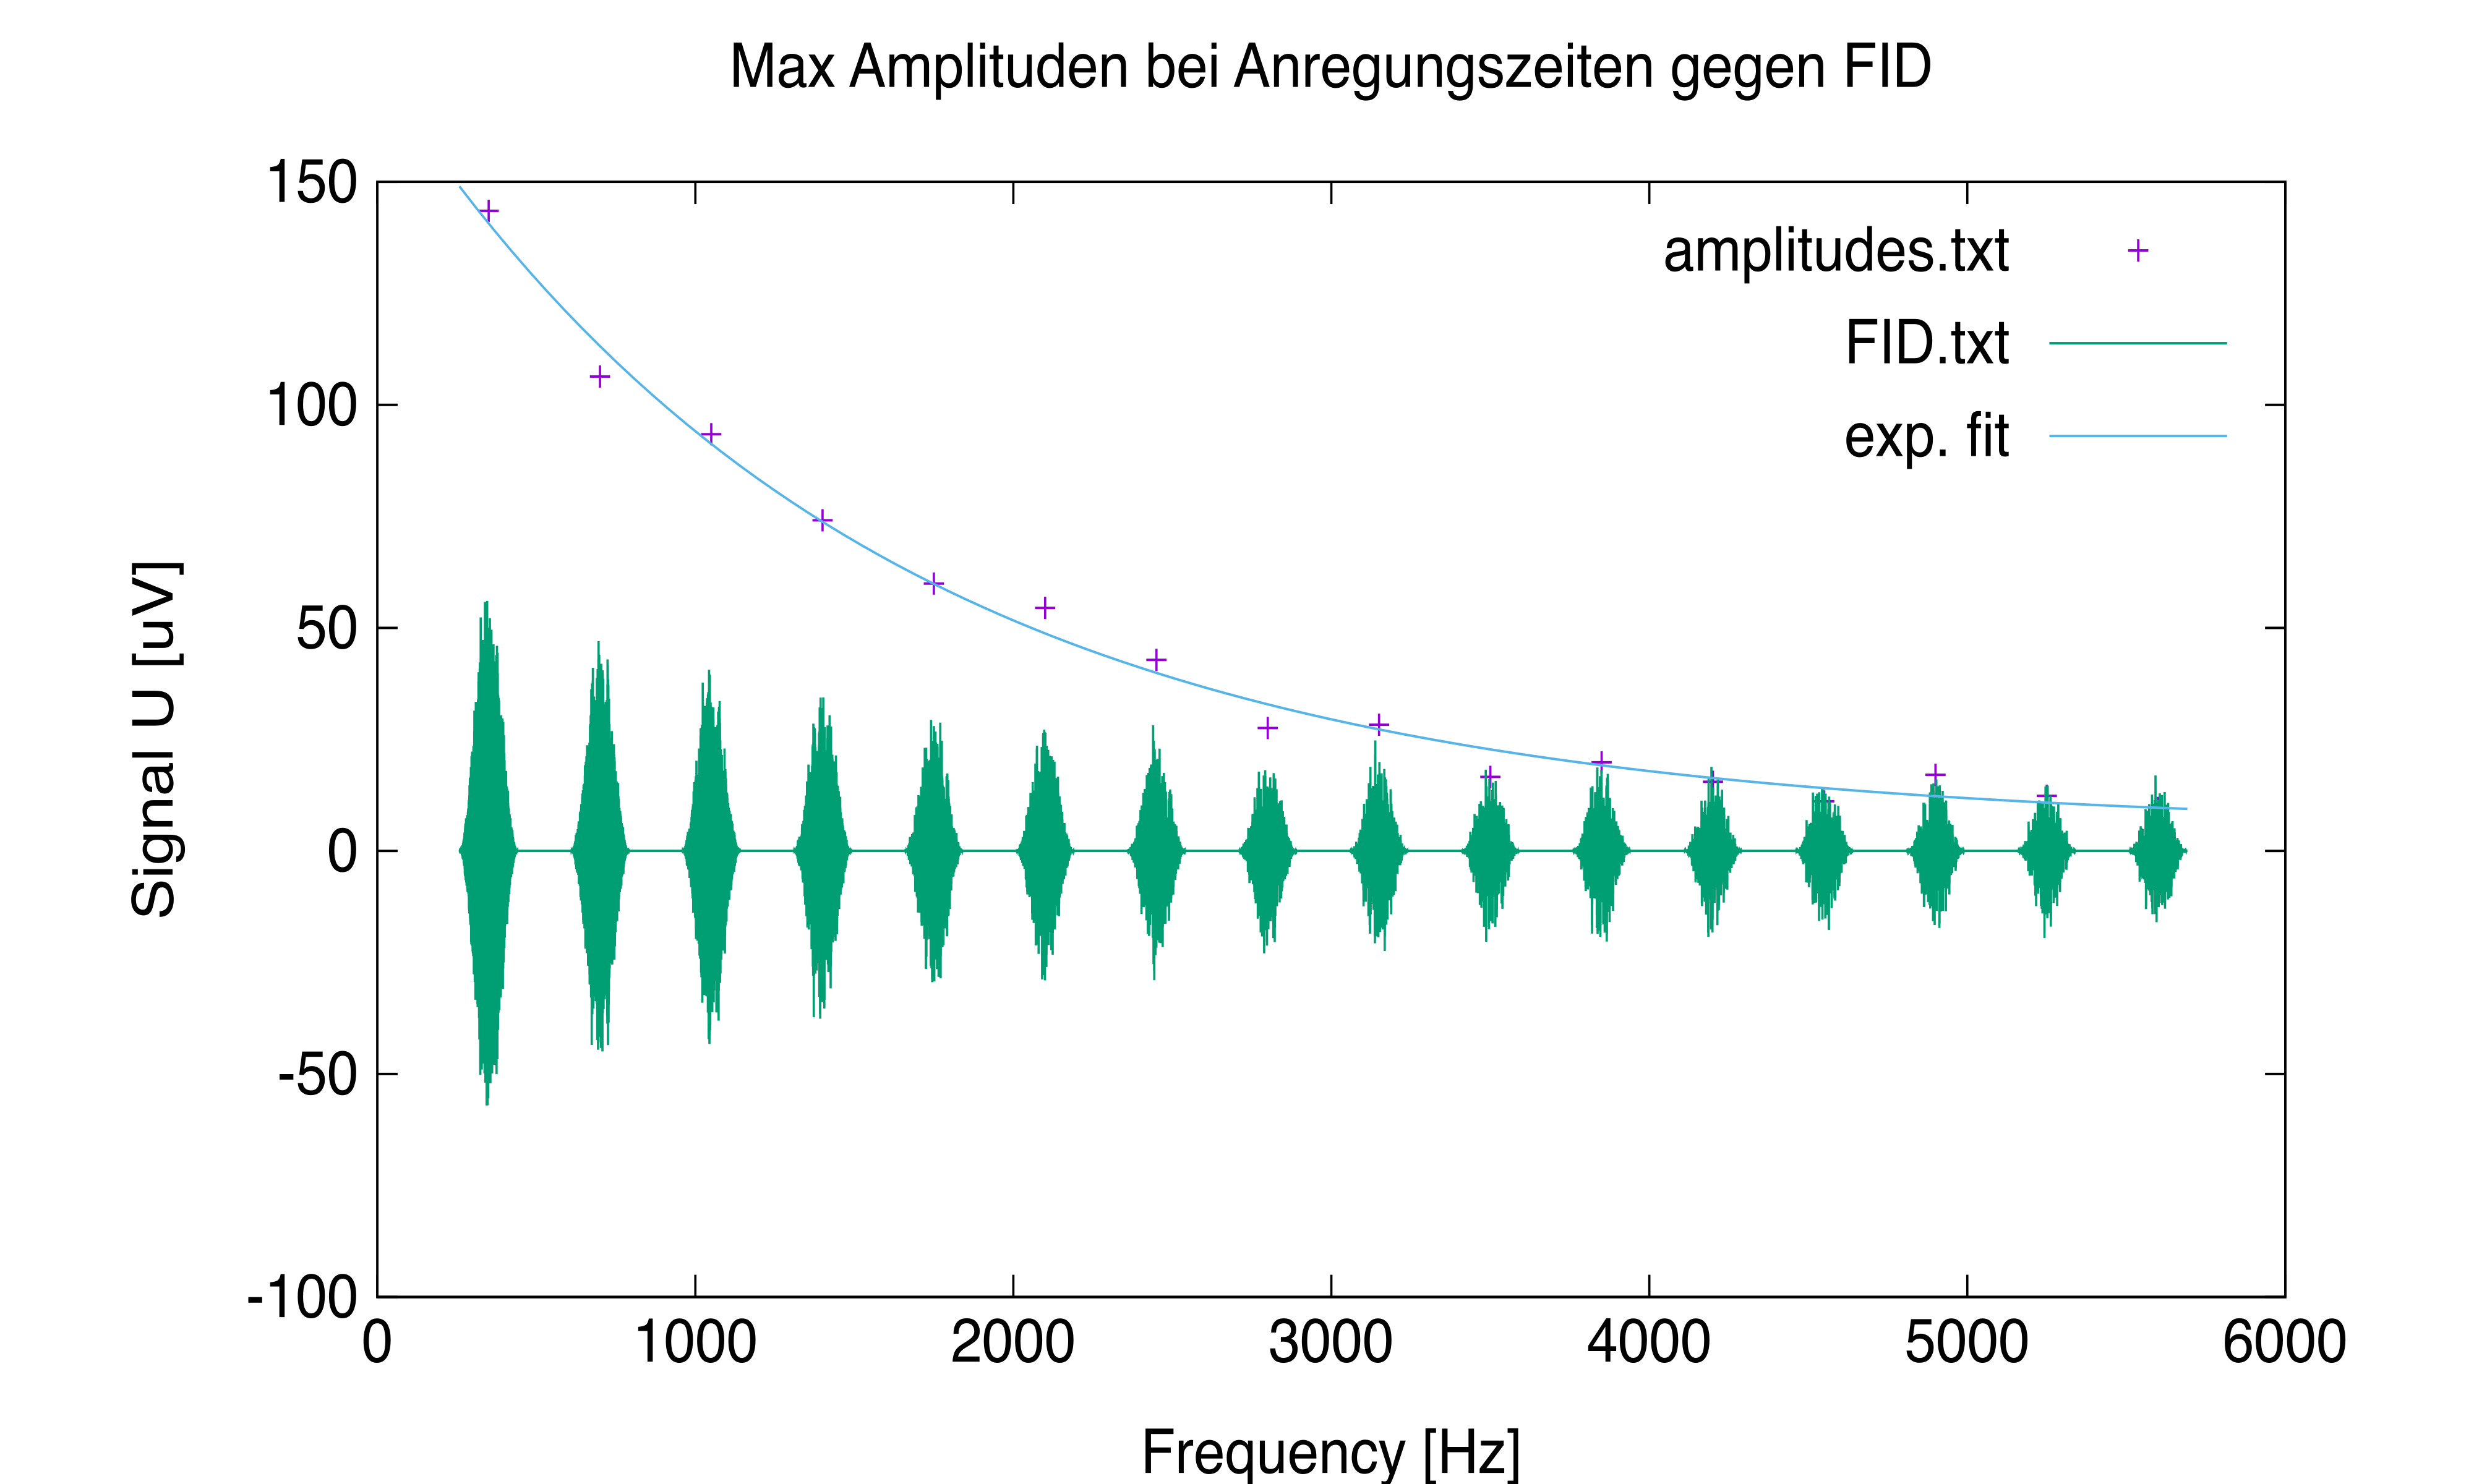
\includegraphics[width=6cm]{Bilddateien/10/CPMG-90-0-constant-avg.png}
                \caption{mod. const.}
                \label{fig:CPMG-90-0-constant-avg}
            \end{subfigure}
            \
            \begin{subfigure}[b]{0.4\textwidth}
                \centering
                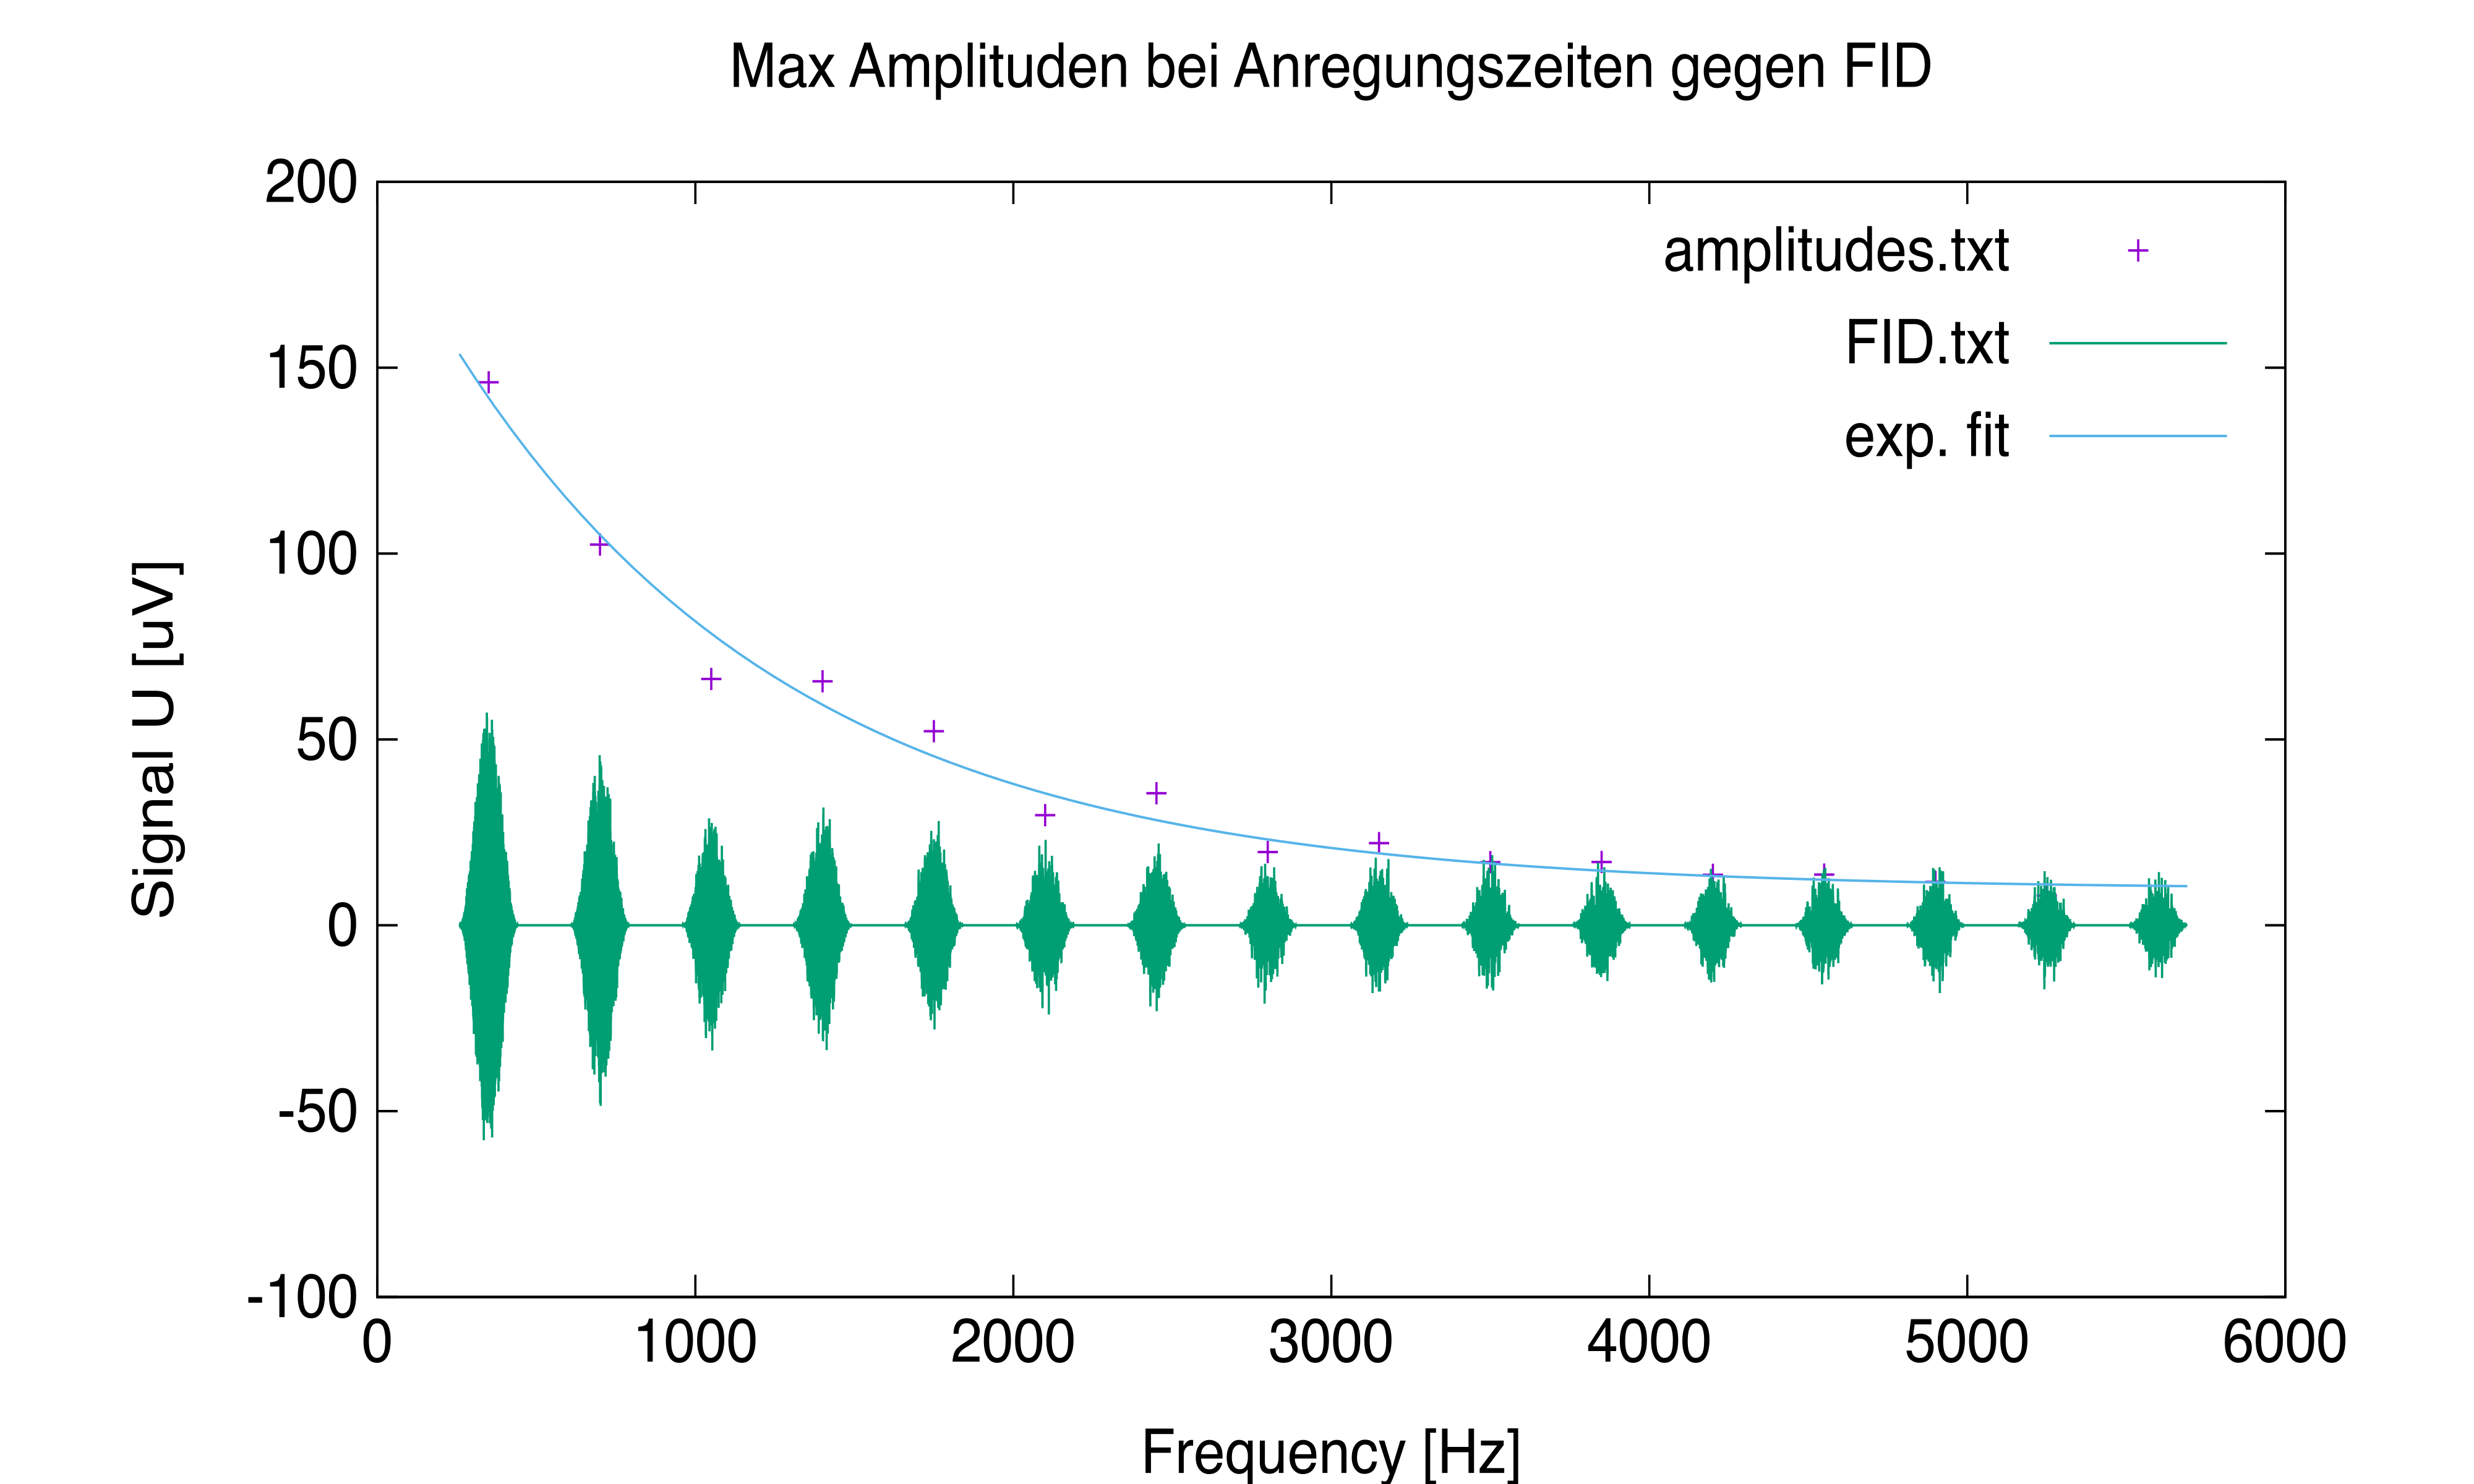
\includegraphics[width=6cm]{Bilddateien/10/CPMG-90-0-alternating-avg.png}
                \caption{mod. alt.}
                \label{fig:CPMG-90-0-alternating-avg}
            \end{subfigure}
            \caption{FID und Amplitudensignale nichtnormiert und gemittelt für $\varphi_1 = 90$, $\varphi_2 = 0$.}
            \label{fig:CPMG-90-0-avg}
        \end{figure}

        \begin{figure}[H]
            \centering
            \begin{subfigure}[b]{0.4\textwidth}
                \centering
                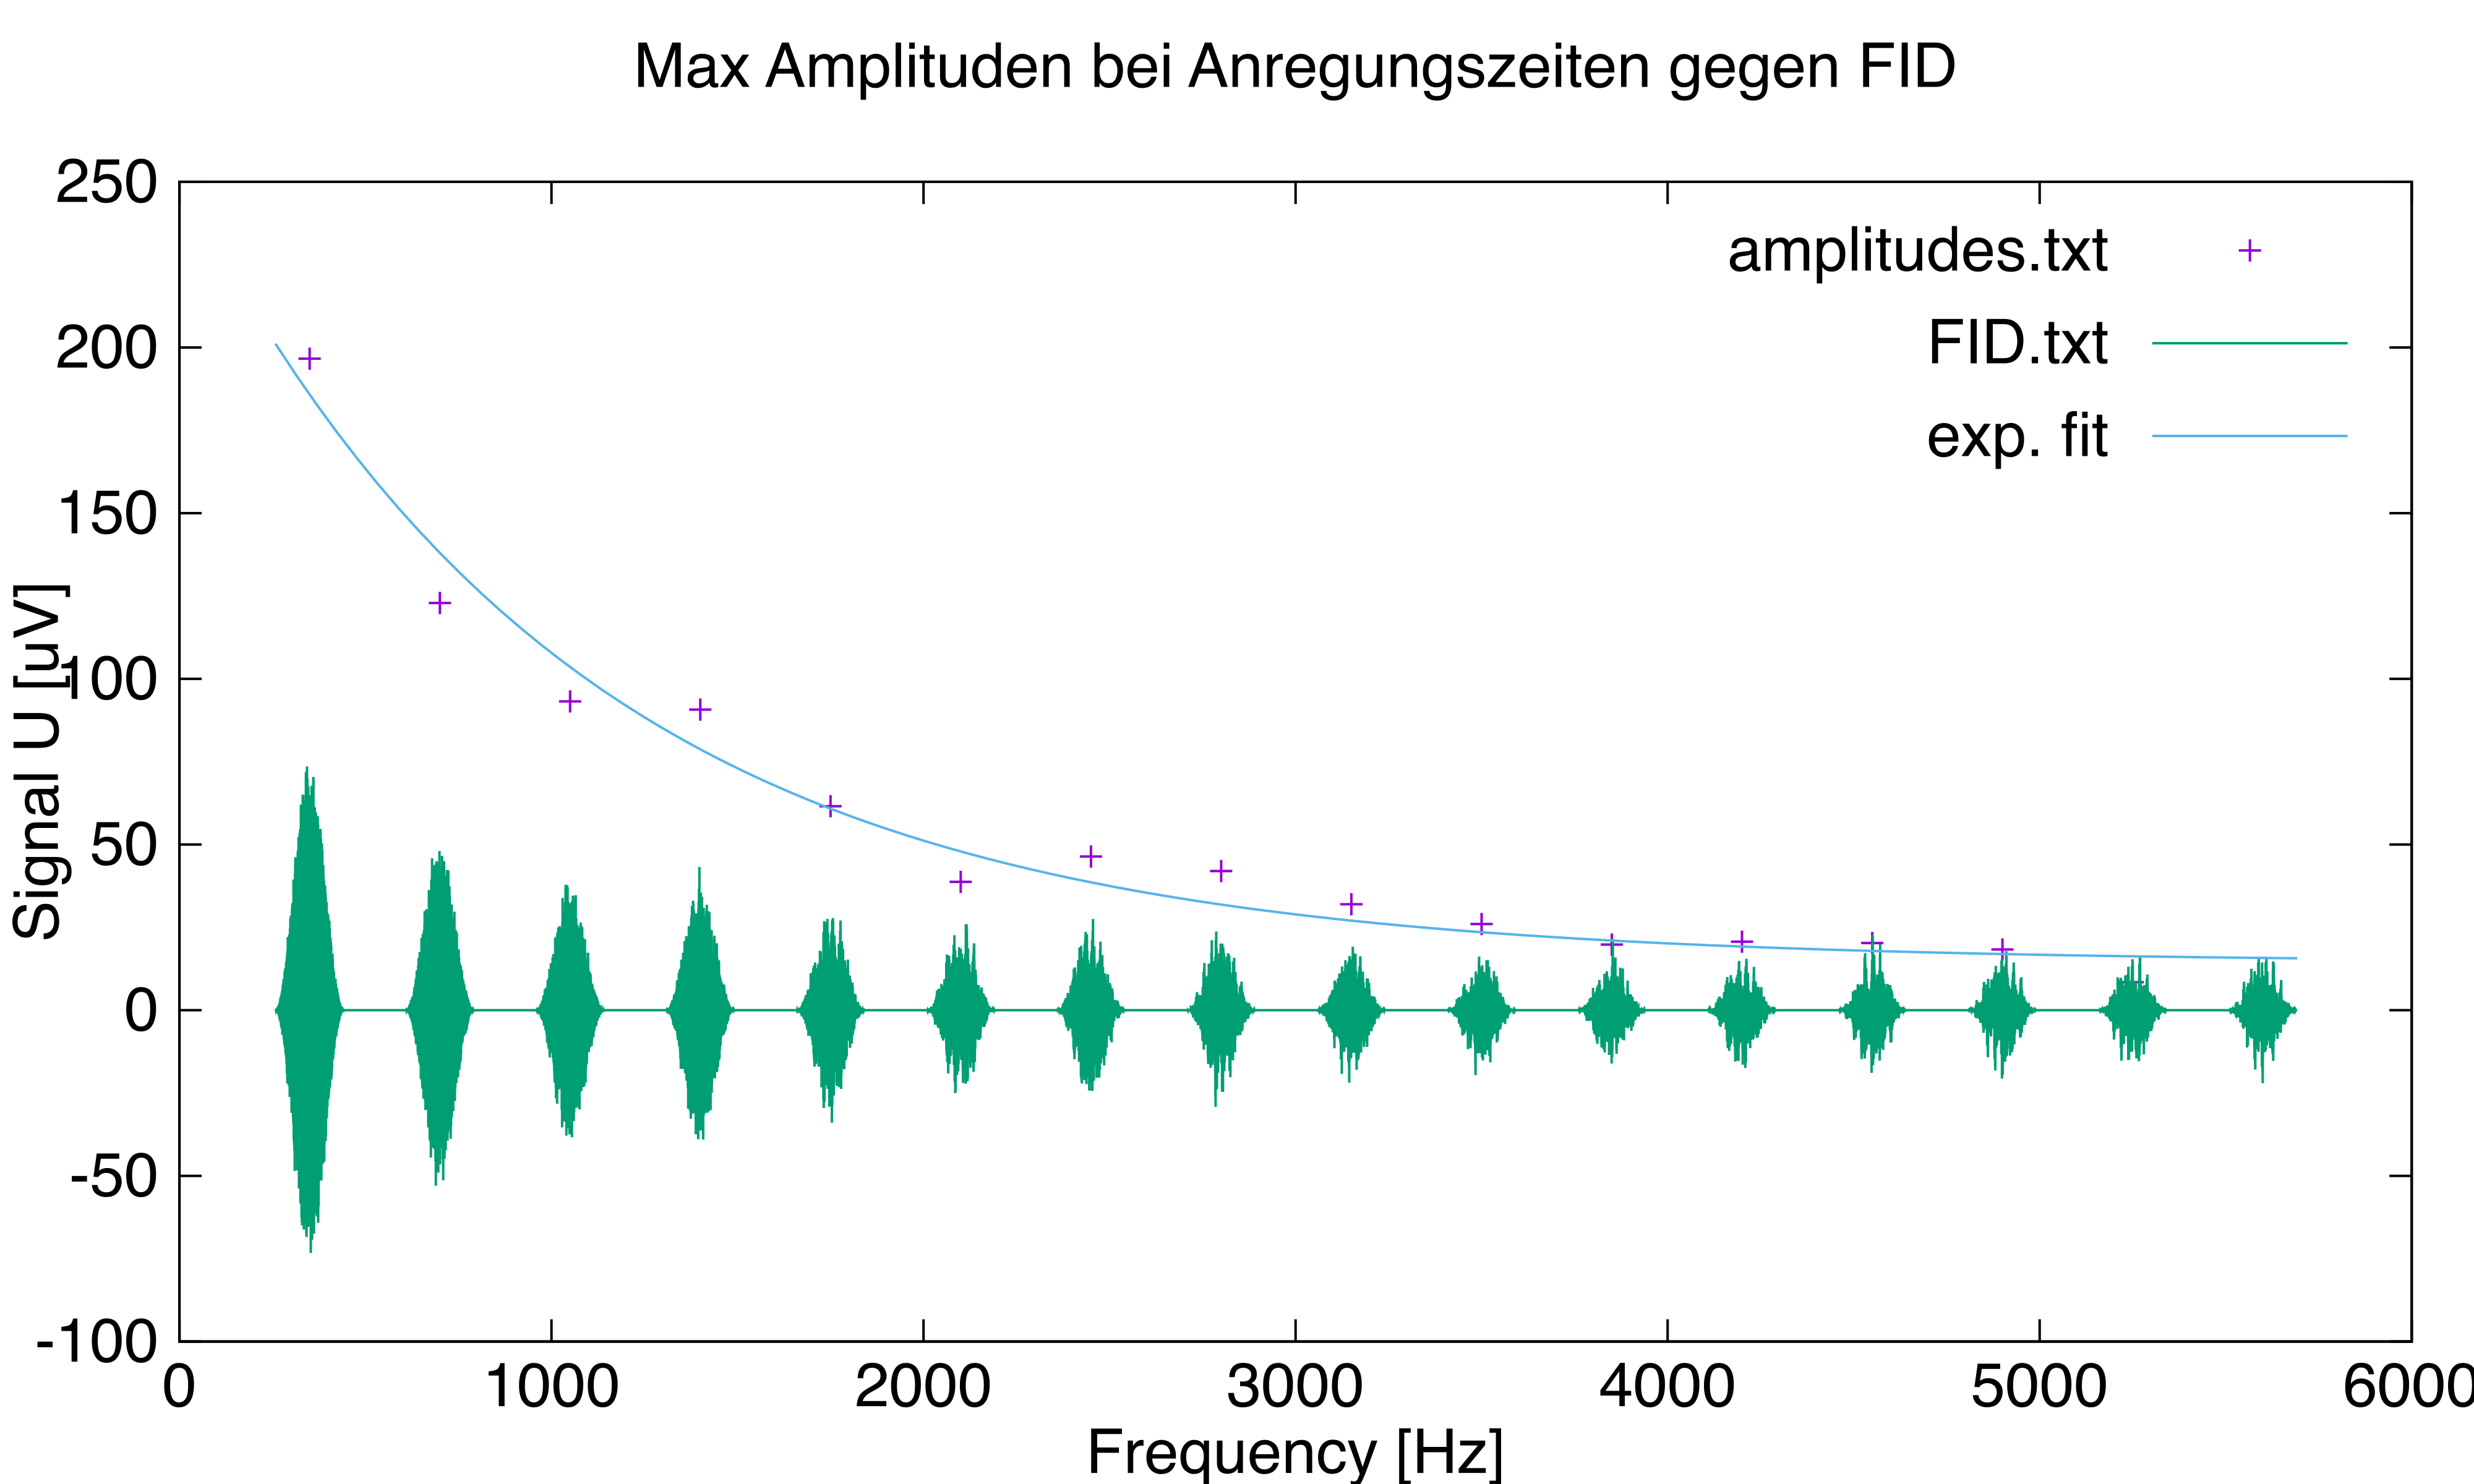
\includegraphics[width=6cm]{Bilddateien/10/CPMG-180-0-constant-avg.png}
                \caption{mod. const.}
                \label{fig:CPMG-180-0-constant-avg}
            \end{subfigure}
            \
            \begin{subfigure}[b]{0.4\textwidth}
                \centering
                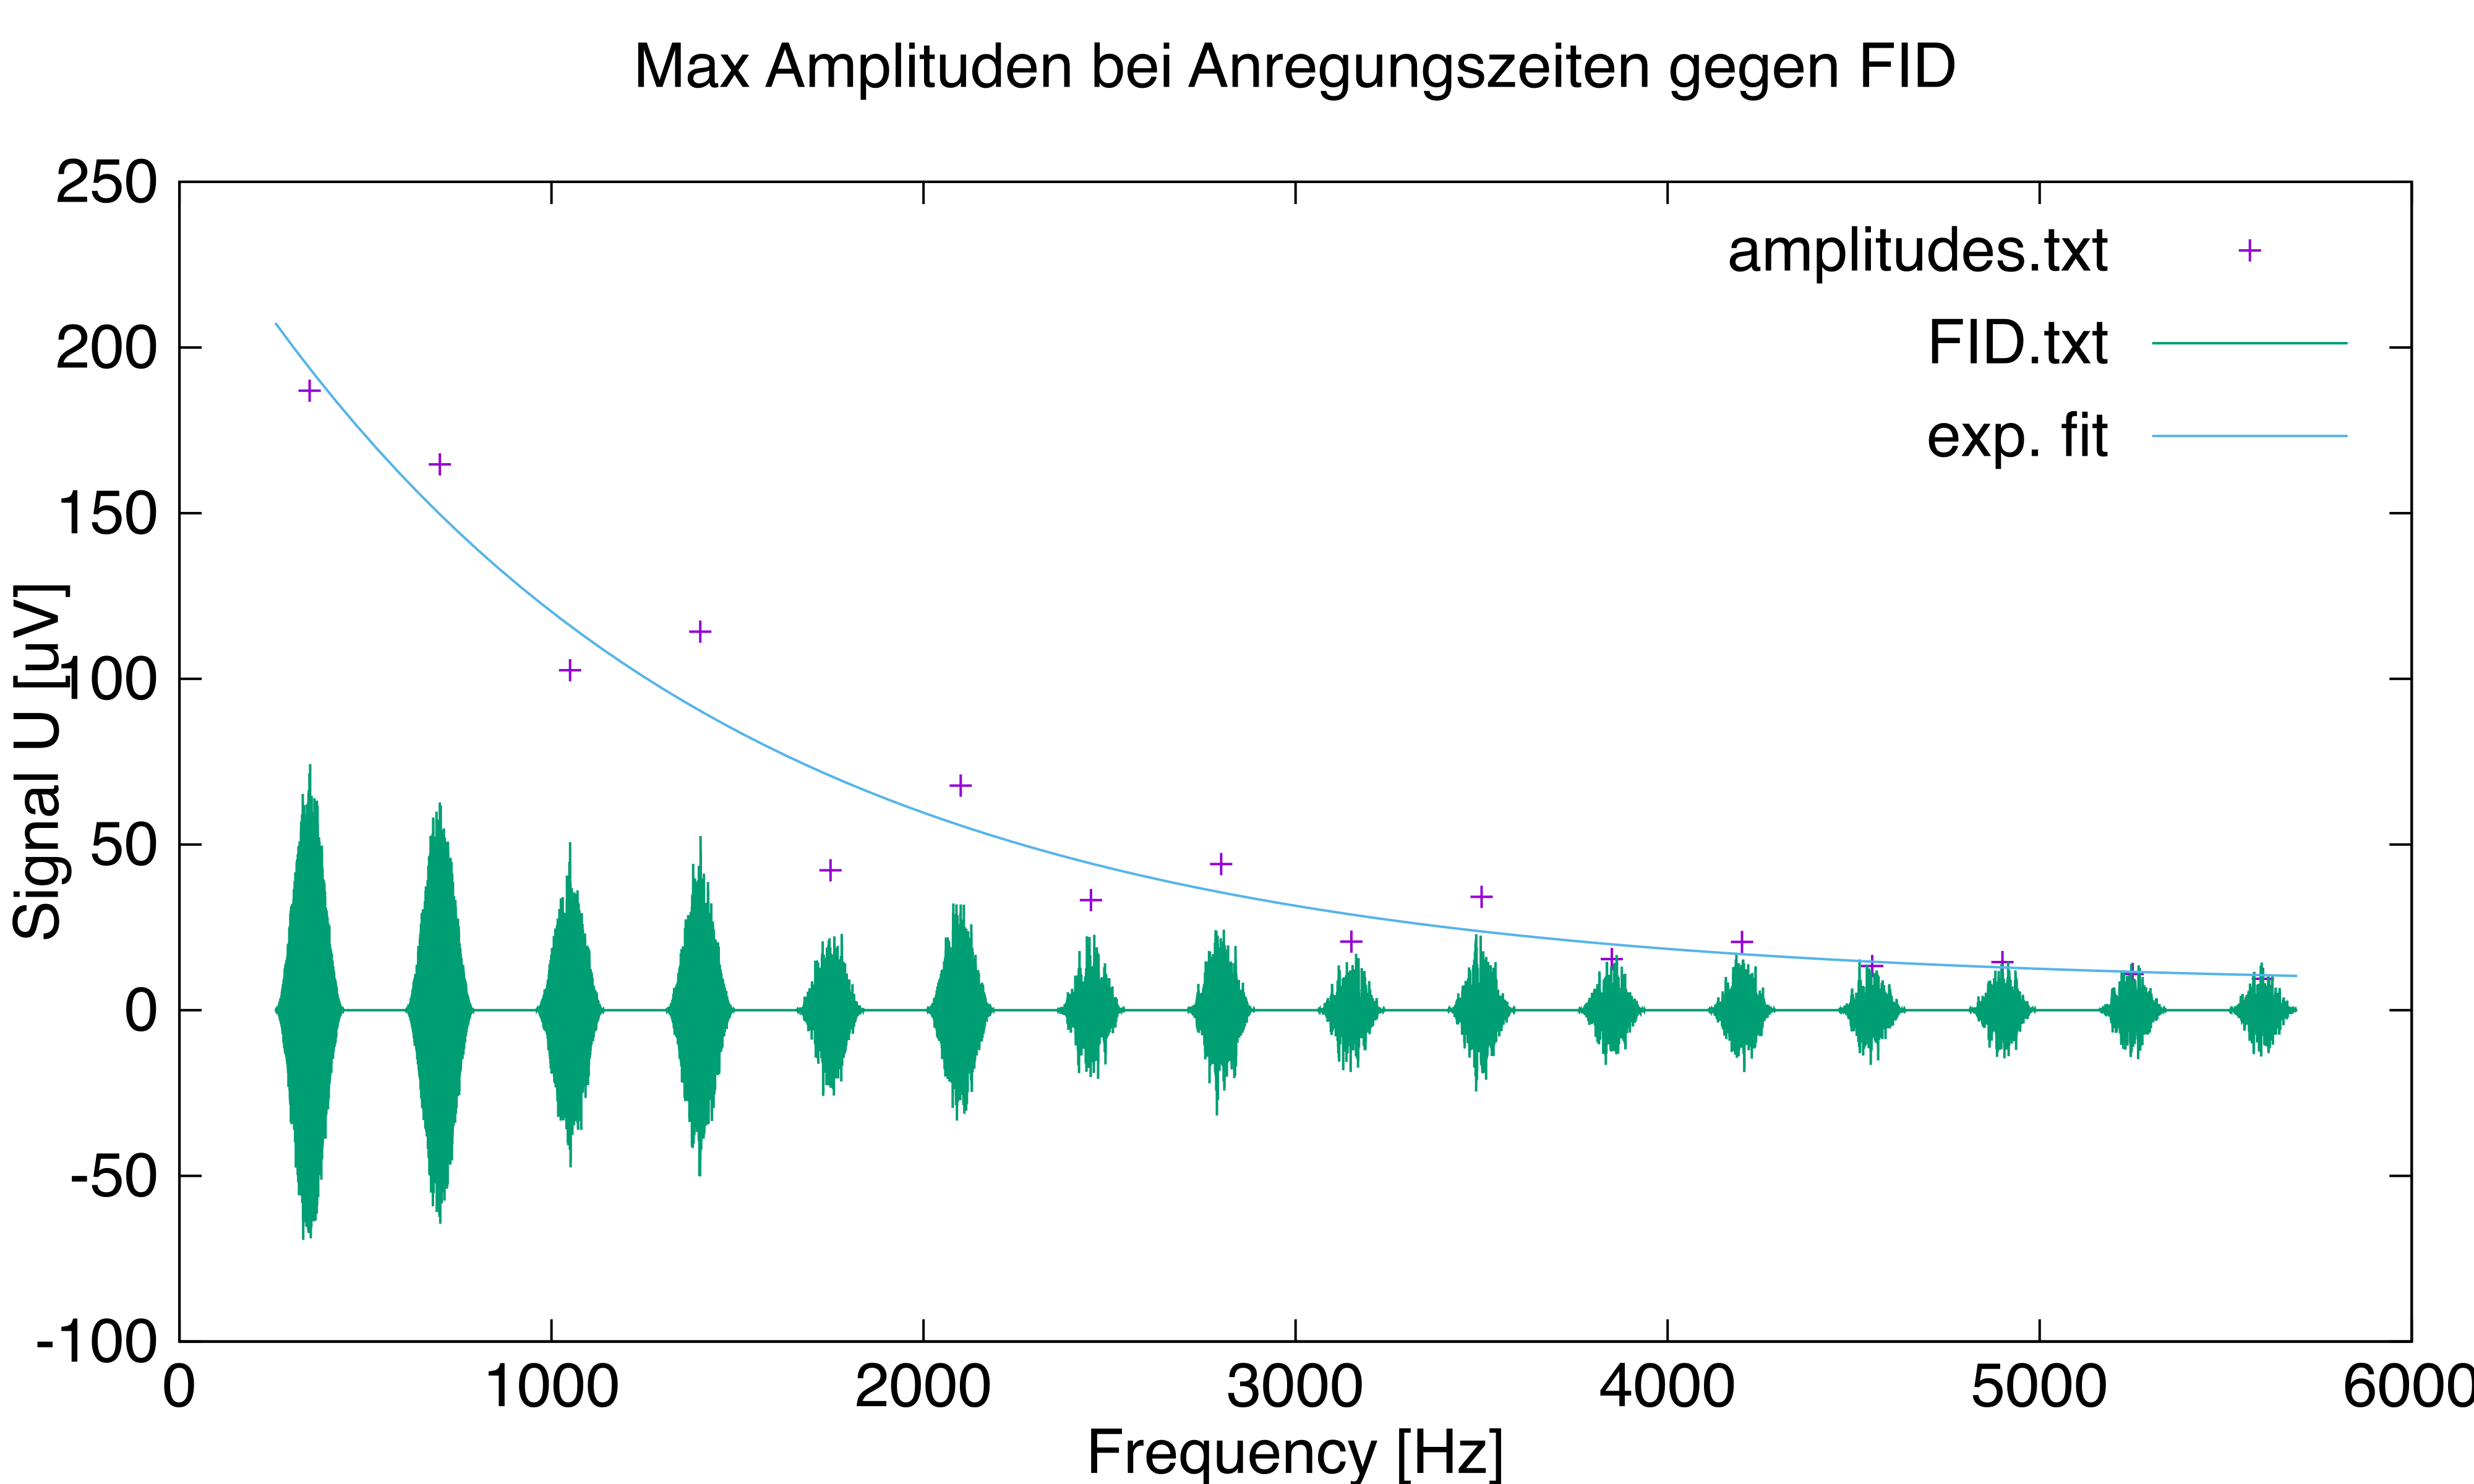
\includegraphics[width=6cm]{Bilddateien/10/CPMG-180-0-alternating-avg.png}
                \caption{mod. alt.}
                \label{fig:CPMG-180-0-alternating-avg}
            \end{subfigure}
            \caption{FID und Amplitudensignale nichtnormiert und gemittelt für $\varphi_1 = 180$, $\varphi_2 = 0$.}
            \label{fig:CPMG-180-0-avg}
        \end{figure}

        \begin{figure}[H]
            \centering
            \begin{subfigure}[b]{0.4\textwidth}
                \centering
                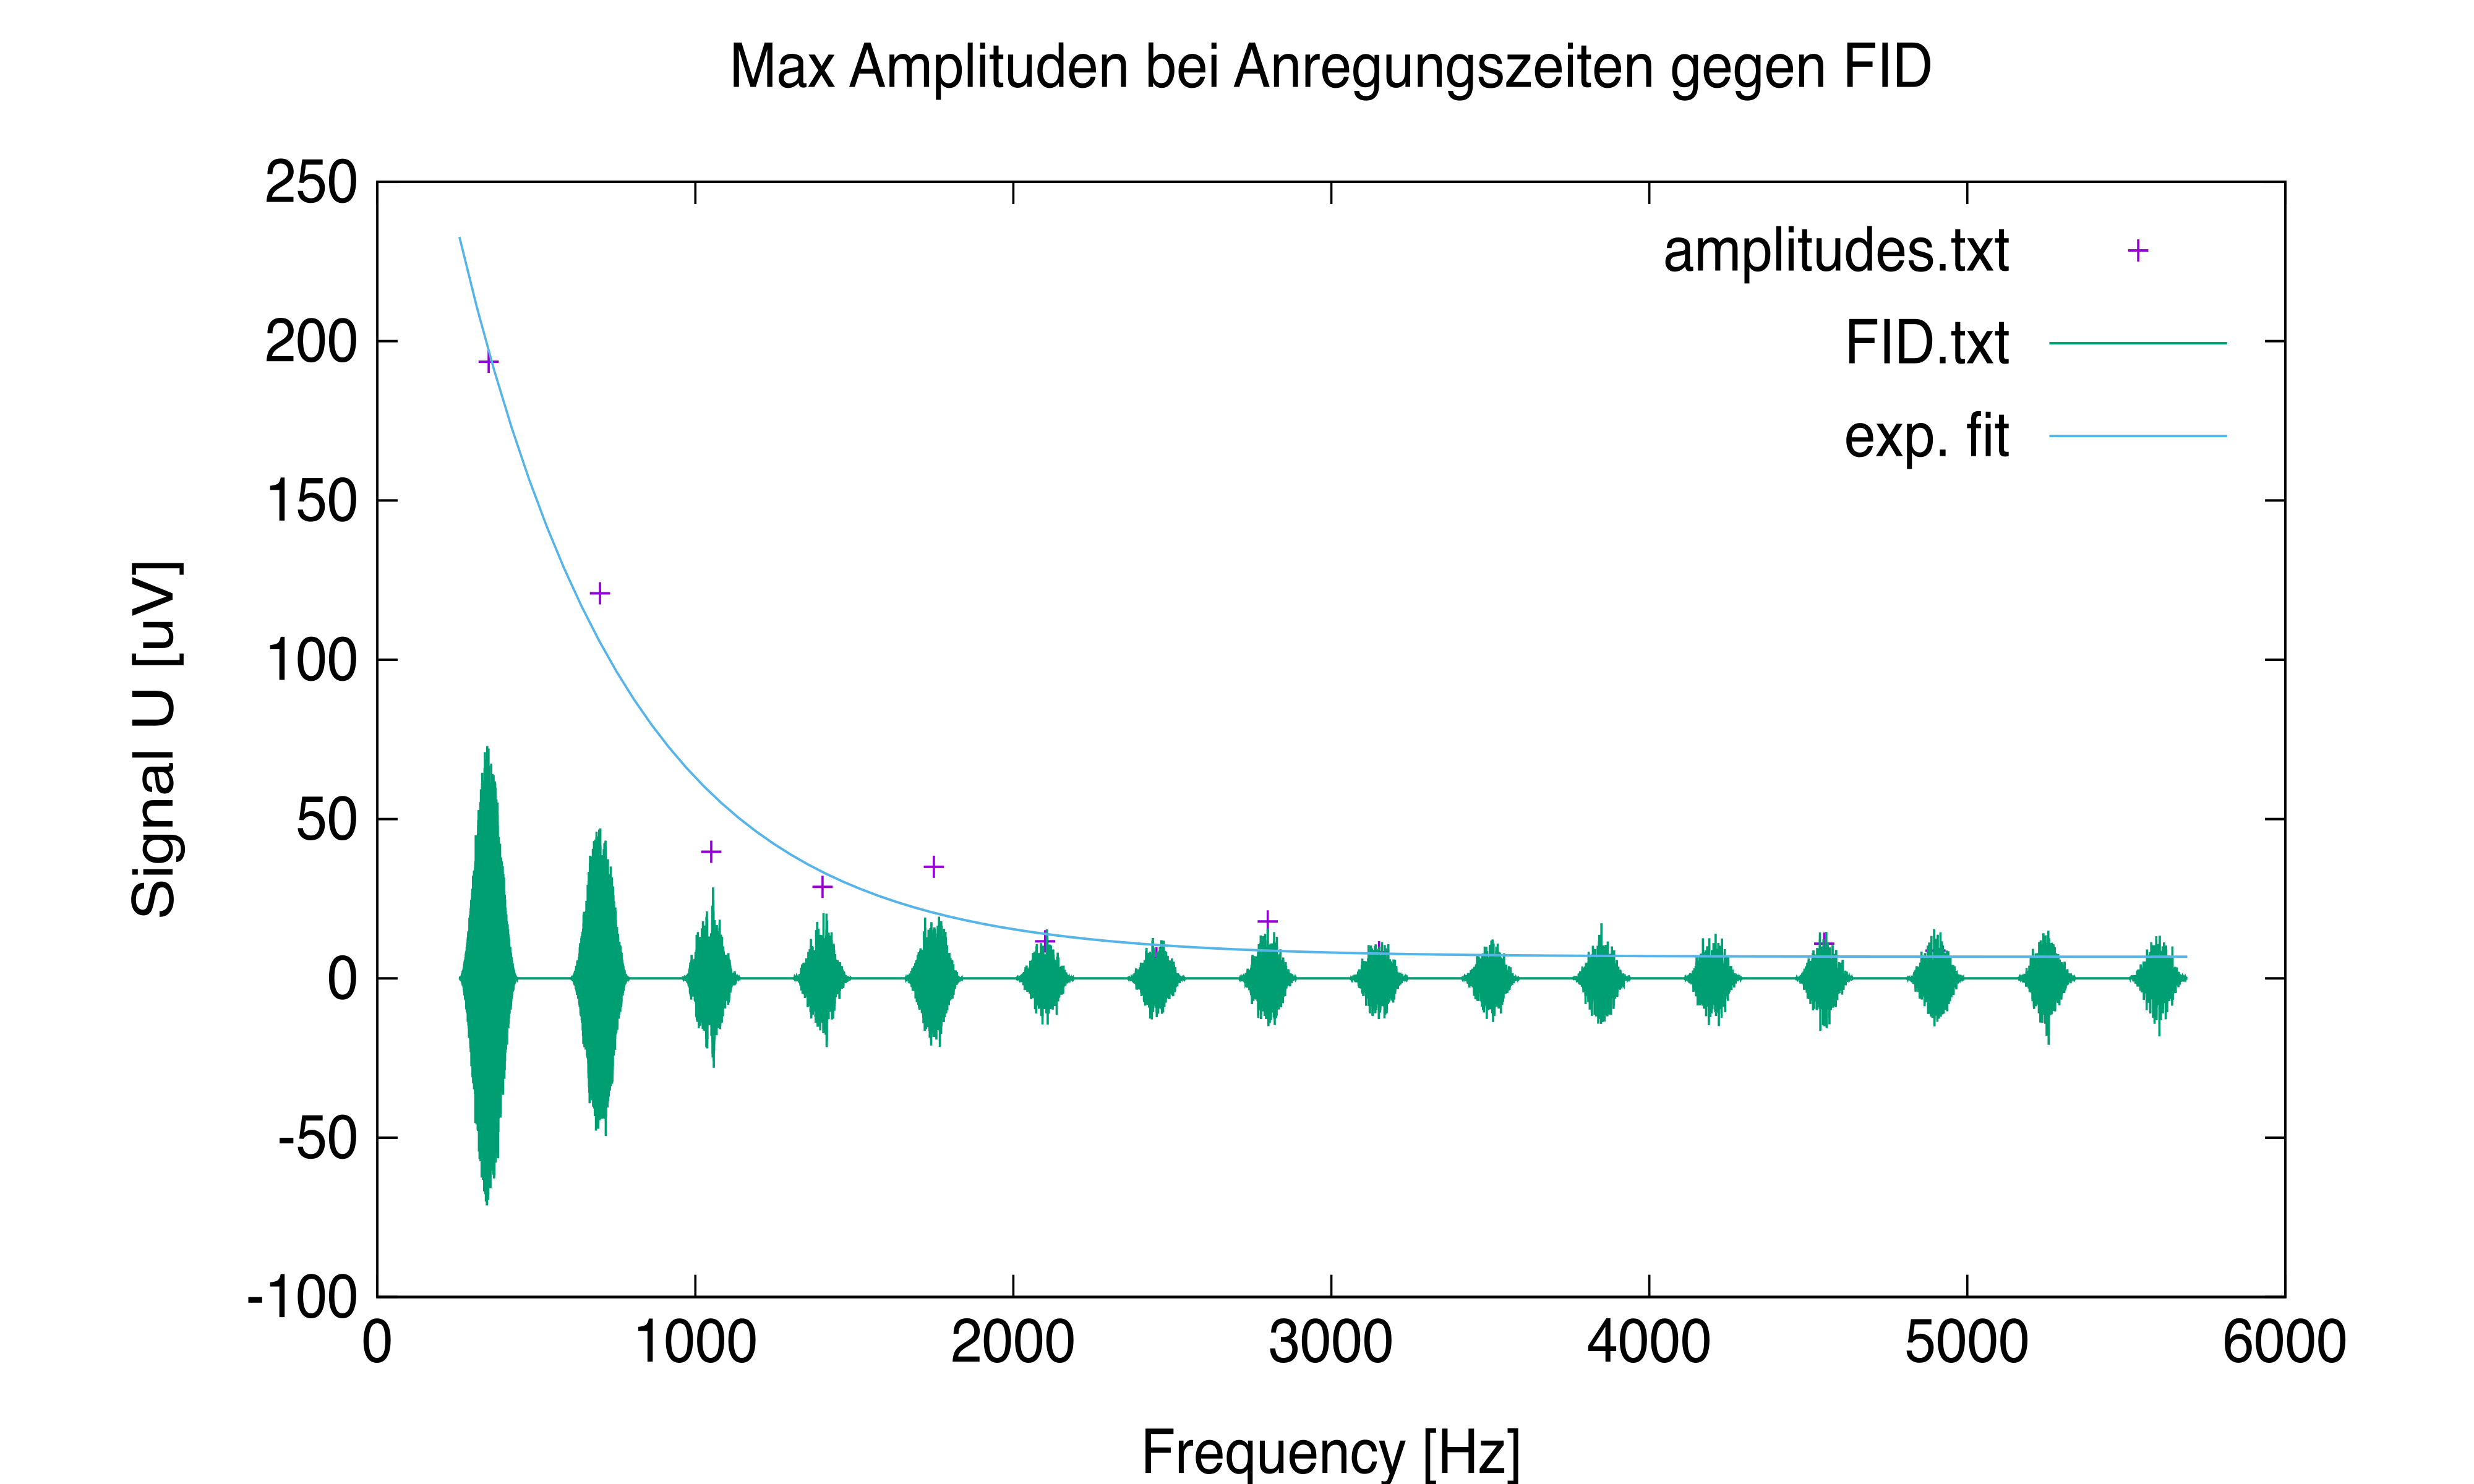
\includegraphics[width=6cm]{Bilddateien/10/CPMG-90-270-constant-avg.png}
                \caption{mod. const.}
                \label{fig:CPMG-90-270-constant-avg}
            \end{subfigure}
            \
            \begin{subfigure}[b]{0.4\textwidth}
                \centering
                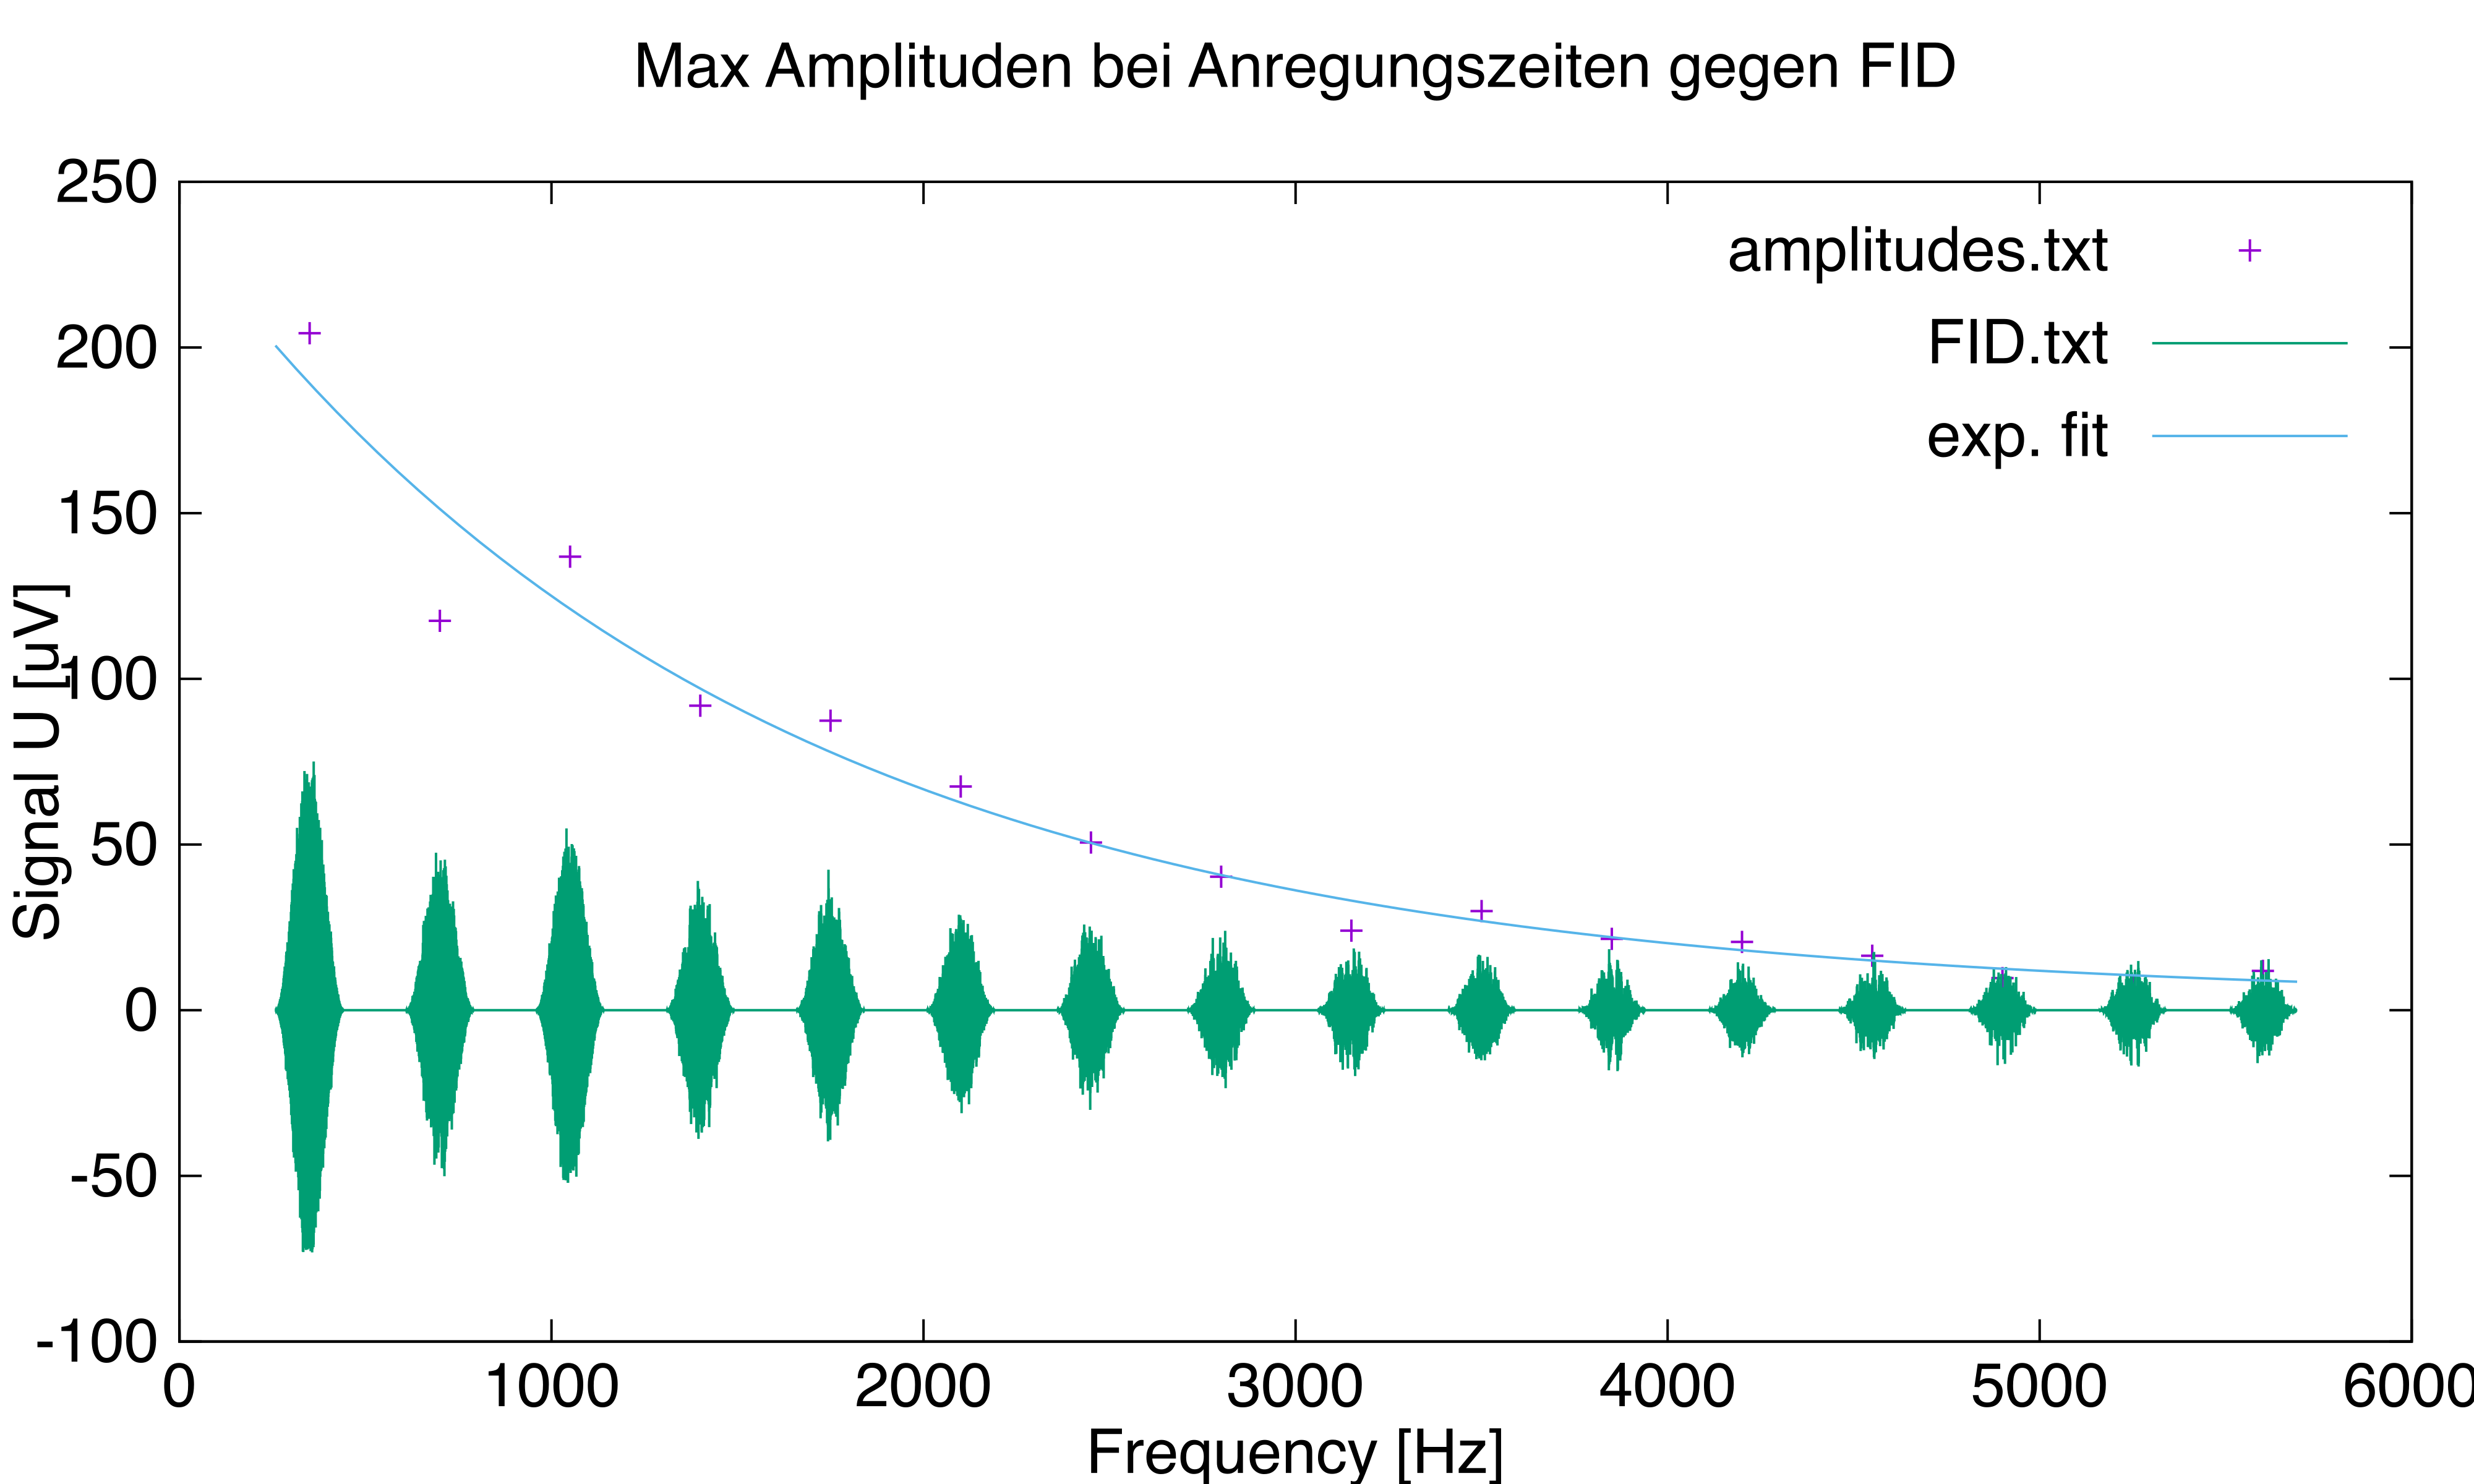
\includegraphics[width=6cm]{Bilddateien/10/CPMG-90-270-alternating-avg.png}
                \caption{mod. alt.}
                \label{fig:CPMG-90-270-alternating-avg}
            \end{subfigure}
            \caption{FID und Amplitudensignale nichtnormiert und gemittelt für $\varphi_1 = 90$, $\varphi_2 = 270$.}
            \label{fig:CPMG-90-270-avg}
        \end{figure}
        

    % \bibliography{../Literatur.bib}
\end{document}